%!TEX root = thesis.tex

\chapter{Interpreting Policies}
\label{chapter5}



\section{Interpretability Background} 

Reinforcement Learning (RL) with deep neural networks has increasingly been used for learning applications due to the ability to solve high-dimensional problems with continuous observation and action spaces. However, the large number of parameters used in the network makes it difficult to develop intuitive interpretations of the logic that governs the policy. This is contrary to conventional controllers which typically describe the relationship between the control output and input with few parameters. In other words, the neural network is a black box which takes observations as its input and provides the actions as the output, but a detailed explanation of the relationship between the observations and corresponding actions is generally unknown.

Post-training methods of interpretation are necessary to provide explanations for the behavior of the agent. Many post-training interpretation methods that have been proposed for image-based agents, where the inputs to the neural networks for the agents consist of pixels from image data rather than the state of a dynamic system~\cite{Alharin:2020a}. Another class of interpretation methods relies on developing high-level summaries of the behavior of the agent~\cite{Lu:2023a}. However, these methods are often time-consuming and require significant manual interpretation.
%
There are not many general methods for providing detailed explanations for low-level agent behavior. One applicable method for low-level interpretation of agents is decision trees~\cite{Bastani:2018a}. Decision trees can be used to distill the deep neural network model onto a shallower model with fewer nodes. The reduction of the model size facilitates developing an intuitive understanding of the behavior of the agent. However, decision trees must be trained from the deep model.
%
Depending on the complexity of the deep neural network model, the decision tree may still contain a significant number of nodes, making it unamenable to interpretation.

This chapter proposes an interpretation method for state-based observations that relies on established control methods to interpret complex policies. The method relies on approximating the agent as a switching controller. The viability of this method was tested on the double-pendulum crane and inverted pendulum benchmark systems.

\section{Interpretable Switching}

There are well established methods for designing linear controllers to provide a linear system with the desired performance characteristics. However, these methods are not directly applicable to nonlinear systems.
One way to simplify controller design for nonlinear systems is to use a set of local controllers designed for subsets of the operating space of the system, where the behavior of the system in a subset of the operating space is easier to describe with linear approximations.
%
% One way to utilize linear control design methods for nonlinear systems is to use a set of linear controllers designed for different local subsets of the system's operating space.
% %
% This can simplify control design and analysis for nonlinear systems.
%
A switching law is then used to combine the individual local controllers into a global control law.
%
One method for designing the local controllers is gain scheduling control, where the form of each local controller is the same, and the gains are updated based on the switching or scheduling rule.
%

The two main types of gain scheduling include discrete scheduling and the Linear Parameter Varying method. For the discrete gain scheduling method, the system is linearized about multiple points in state-space; gains of a state feedback controller are then selected to provide desirable performance when the system is near that linearization point~\cite{Hyde:1993a,Leith:2000a}. This forms a type of piecewise controller for different regions of the workspace. Since this makes discrete regions in the state space where the gains are fixed, the gains are often interpolated between the different regions. It is also possible to use Linear Parameter Varying control to generate a continuous switching law for the gains~\cite{Rugh:2000a,Hoffmann:2015a}.
%
In gain scheduling control, a single scheduling variable is often used to indicate when to switch from one set of gains to another~\cite{Shamma:1990a}. To be effective, this scheduling variable needs to be meaningful and capture the nonlinearity of the system. 

Although gain-scheduling and switching control are usually used to simplify controller design for nonlinear systems, this work proposes using local approximations of RL agents to improve interpretability.
%
By fitting local behaviors of the black-box agent to local approximations with few parameters, the behavior of the agent in a subregion of state space can be more easily understood. A more general understanding of the behavior of the agent can then be developed by consolidating the interpretations of the local approximations.
%
There are multiple challenges with representing an agent with a switching controller. The local controller will need to approximate the input-output law of the agent for a subset of the observation space. However, there can be error in the local approximations of the agent in each subset of state space, which may lead to significant error in the time response.
% The goal is to minimize the error between the agent output and the output of each local controller.
Factors that contribute to the accuracy of the fit include using an appropriate scheduling variable, an appropriate fit function, and an appropriate number of local control functions.

The local approximations in the piecewise controllers were generated by minimizing the error between the agent's output and the output of the local controller. Each local controller approximates the output of the agent for a subset, $s_l$, of all possible states, $\mathbb{S}\subset\mathbb{R}^n$, where $n$ is the system order.
% The set of all sampled states for which the piecewise controller is defined as $\mathbb{S}=\{s_1, s_2, \dots, s_l\}$.
% Each local controller is generated for a subset, $s_l \subset \mathbb{S}$.
The subset, $s_l$, is defined for a range of the scheduling variable. A local approximation is then generated by:
%
\begin{equation}
\text{minimize} \quad u(s) - \hat{u}_l(s) \quad \forall s \in s_l
\end{equation}
%
where $u(s)$ is the output from the agent controller for an input state, $s$, and $\hat{u}_l(s)$ is the output of the local approximation. The local approximations are then collected to form $\hat{u}(s)$, which approximates the agent $\forall s \in \mathbb{S}$.
% It is important to note that the piecewise approximation is only generated for the agent.
For the combined controllers, the conventional control components remain unchanged while the RL agent components are replaced with the piecewise local approximations.
%

\section{Model Verification}

After generating the switching controller approximations, it is necessary to verify the accuracy of the approximations in terms of time-based performance to determine the trustworthiness of the approximation for interpreting the agents.
This work uses Integral Square Error (ISE) of the time responses from the agent controllers and switching controller approximations:
%
\begin{equation}
ISE = \int_0^T (y(t) - \hat{y}(t))^2 \, \text{d}t
\label{eq_chap5:ISE_func}
\end{equation}
%
where $y(t)$ is the output from the response with the agent controller, and $\hat{y}(t)$ is the responses from the approximate switching controller. ISE provides a single measurement to quantify the response error between the response with the agent and the responses with the switching controller. However, the ISE will depend on the initial condition, so the ISE must be evaluated for an adequate number of samples to evaluate the accuracy of the switching controller.

\section{Interpreting Combined Controllers}

\subsection{Double-Pendulum Crane Agent Approximation}

This section presents an analysis of switching controllers for the double-pendulum crane shown previously in Chapter~\ref{chapter2}. Multiple switching controllers with different numbers of local approximations were generated for the Pure RL and combined controllers.
As a reminder, the controllers trained for the double-pendulum crane were:
%
\begin{align*}
&\qquad\qquad\text{Pure RL:} & u&=a_t \qquad\qquad\qquad\\
&\qquad\qquad\text{RL-PD:} & u&=k_px+k_d\dot{x} + \boldsymbol{a}_t\boldsymbol{\theta} \qquad\qquad\qquad\\
&\qquad\qquad\text{RL-LA:} & u&=k_px+k_d\dot{x} + a_t \qquad\qquad\qquad\\
&\qquad\qquad\text{RL-PD-LA:} & u&=k_px+k_d\dot{x} + \boldsymbol{a}_t\boldsymbol{\theta} + a_t \qquad\qquad\qquad
\end{align*}
%
where $u$ is the desired acceleration command for the crane trolley. Pure RL is a controller using just the action, $a_t$, as the output. RL-PD has fixed-gain terms on the trolley states as well as gain scheduled terms on pendulum states. RL-LA has the fixed-gain component and a single, lumped action. RL-PD-LA has fixed-gain terms, gain scheduling, and lumped action.
%
The inputs for the local controllers are the same as the neural network policies, which are the displacement and velocities of the trolley, hook, and payload of the crane.
% \rph{The local controllers accept the same inputs as the neural network policies, which is the state of the crane.}
% The inputs for each local controller match the observation space for the crane during training, which is the state of the crane.
Polynomials are commonly used for general curve fitting applications and are used here to generate local approximations of the behavior of the agent:
% A polynomial function was used to curve fit the agent for each local controller:
%
\begin{equation}
    \hat{a}_l=\sum_{i=1}^p a_ix^i + b_i\dot{x}^i + c_i\theta_1^i + d_i\dot{\theta_1}^i + e_i\theta_2^i + f_i\dot{\theta_2}^i
\label{eq_chap5:dpcrane_approx_func}
\end{equation}
%
where $l$ is the current local controller, and $p$ is the degree of the polynomial, $x$ and $\dot{x}$ are the trolley displacement and velocity, $\theta_1$ and $\dot{\theta}_1$ are the angular displacement and angular velocity of the hook, and $\theta_2$ and $\dot{\theta}_2$ are the angular displacement and angular velocity of the payload. Although polynomials of higher degree provide the potential to generate more accurate approximations, the increase in the number of parameters in each local controller can decrease interpretability. Therefore, the polynomial degree selected for the crane controller approximations was $p=3$.
%
The most vital function of the crane is to move the trolley to the desired displacement. Therefore, the scheduling variable used to switch between the local controllers is the displacement of the crane trolley.

%
Figure~\ref{fig_chap5:dpcrane_trolley_unclipped_approx_error} shows the ISE of the trolley responses for two sets of switching controllers using one and five local approximations.
The ISE is measured for a range of initial values of the scheduling variable. Since multiple agents were trained for each controller type, the lines in the figures show mean ISE and the shaded region shows the standard deviation of the ISE for the responses. The solid gray vertical lines show the switching boundaries for the local approximations.
%
Both sets of approximations are able to maintain low response error. However, the error from the approximations with only 1 local controller, shown in Figure~\ref{subfig_chap5:dpcrane_trolley_unclipped_approx_error_1_bins}, has smoother trends than the ISE from five local approximations in Figure~\ref{subfig_chap5:dpcrane_trolley_unclipped_approx_error_5_bins}. Increasing the number of local approximations tends to increase the magnitude of the peaks in ISE, where each peak is also associated with higher variance in ISE. Although generating local approximations from smaller subsets may provide less error between the approximation and the agent, switching sometimes creates instability in the responses.
%
\begin{figure}[t]
    \centering
    \begin{subfigure}[b]{0.49\textwidth}
        \centering
        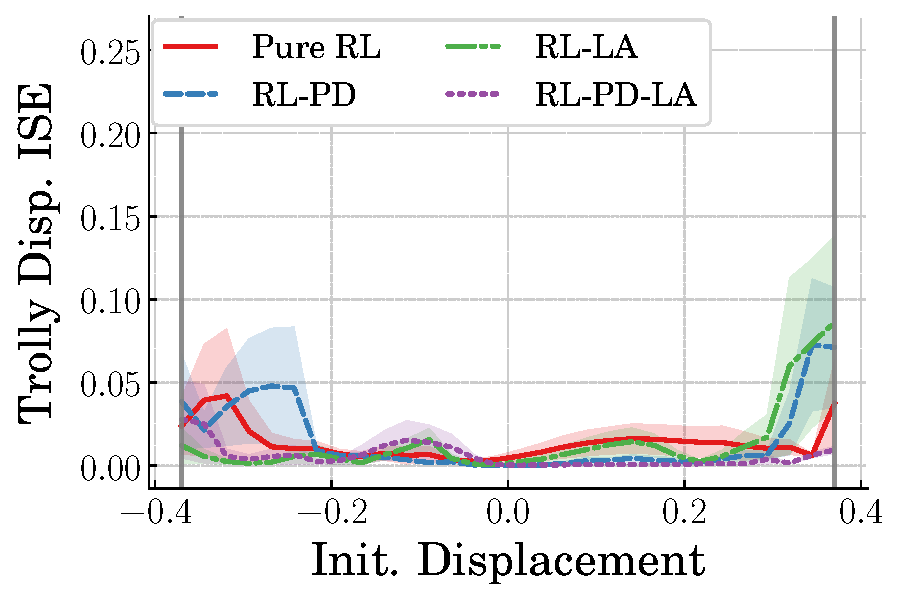
\includegraphics[width=\textwidth]{figures/figures_Interpretability/Mean_ISE_dpcrane_cubic_1_bins/Mean_ISE_dpcrane_cubic_Trolly_Disp_1_bins.pdf}
        \caption{1 local approximation}
        \label{subfig_chap5:dpcrane_trolley_unclipped_approx_error_1_bins}
    \end{subfigure}
    \hfill
    \begin{subfigure}[b]{0.49\textwidth}
        \centering
        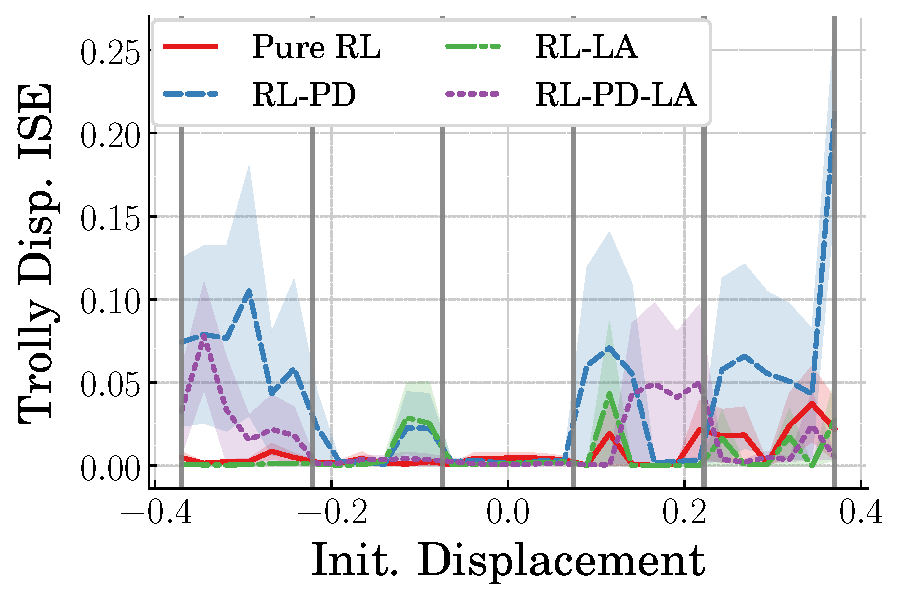
\includegraphics[width=\textwidth]{figures/figures_Interpretability/Mean_ISE_dpcrane_cubic_5_bins/Mean_ISE_dpcrane_cubic_Trolly_Disp_5_bins.pdf}
        \caption{5 local approximations}
        \label{subfig_chap5:dpcrane_trolley_unclipped_approx_error_5_bins}
    \end{subfigure}
       \caption{ISE of crane trolley for local controllers}
       \label{fig_chap5:dpcrane_trolley_unclipped_approx_error}
\end{figure}

%
\begin{figure}
    \centering
    \begin{subfigure}[b]{0.32\textwidth}
        \centering
        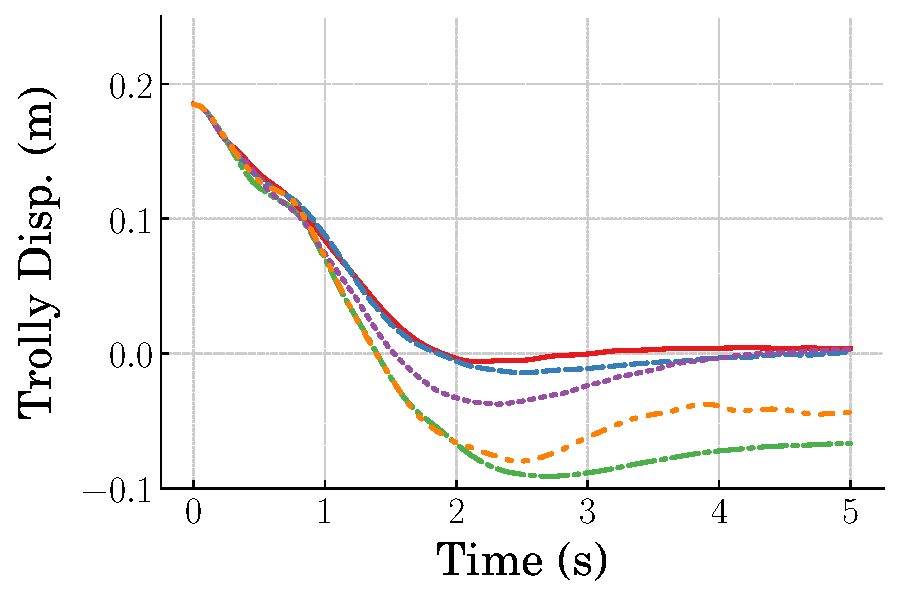
\includegraphics[width=\textwidth]{figures/figures_Interpretability/Mean_ISE_dpcrane_cubic_1_bins/curve_fit_time_responses/pure_RL/agent_0p18_Trolly_Disp.pdf}
        \caption{Agent response}
        \label{subfig_chap5:dpcrane_pure_RL_trolley_0.185_init_agent_unclipped}
    \end{subfigure}
    \hfill
    \begin{subfigure}[b]{0.32\textwidth}
        \centering
        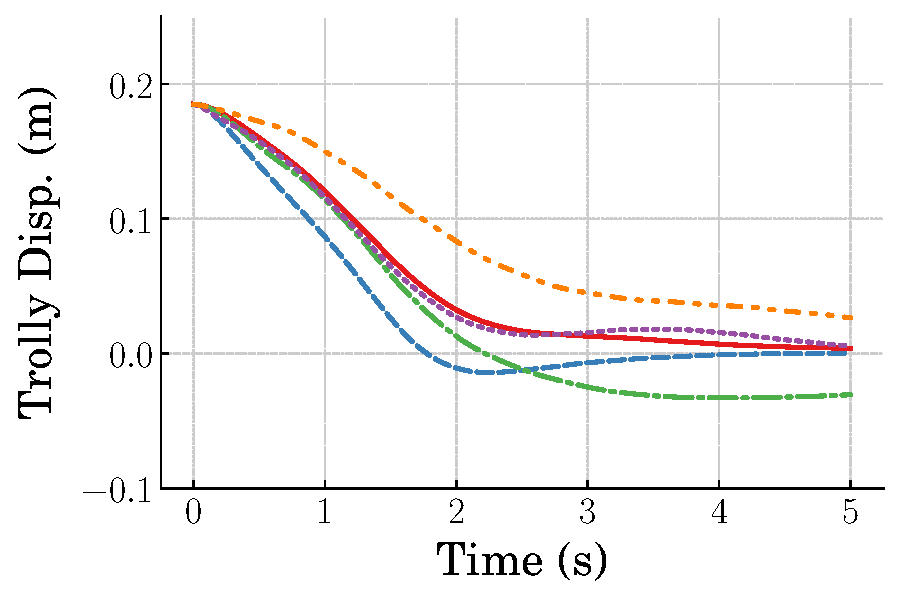
\includegraphics[width=\textwidth]{figures/figures_Interpretability/Mean_ISE_dpcrane_cubic_1_bins/curve_fit_time_responses/pure_RL/curve_fit_0p18_Trolly_Disp.pdf}
        \caption{1 local approximation}
        \label{subfig_chap5:dpcrane_pure_RL_trolley_0.185_init_curve_fit_1_bins_unclipped}
    \end{subfigure}
    \hfill
    \begin{subfigure}[b]{0.32\textwidth}
        \centering
        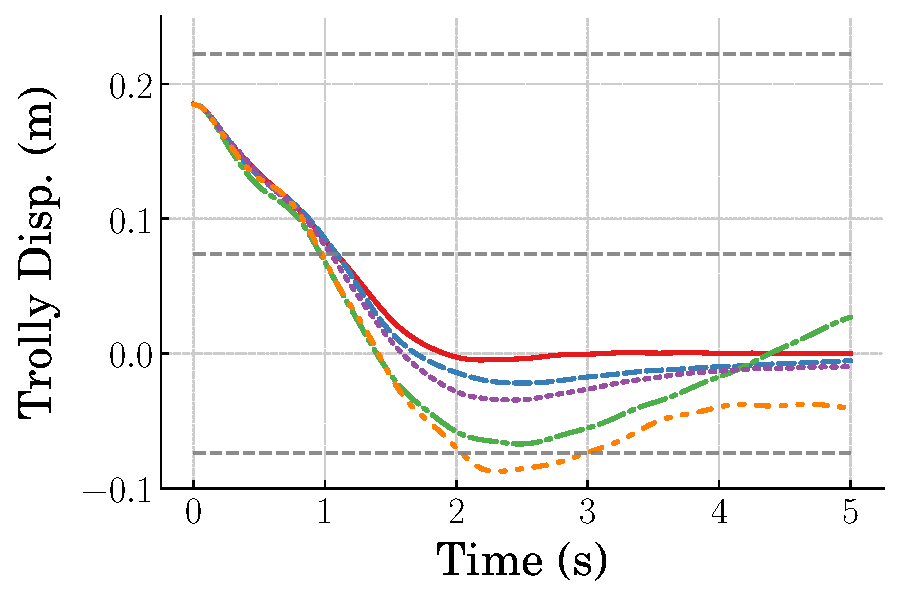
\includegraphics[width=\textwidth]{figures/figures_Interpretability/Mean_ISE_dpcrane_cubic_5_bins/curve_fit_time_responses/pure_RL/curve_fit_0p18_Trolly_Disp.pdf} 
        \caption{5 local approximations}
        \label{subfig_chap5:dpcrane_pure_RL_trolley_0.185_init_curve_fit_5_bins_unclipped}
    \end{subfigure}
    \hfill
    \caption{Pure RL curve fit responses for crane trolley for $x(0)=0.185\si{\meter}$}
    \label{fig_chap5:dpcrane_pure_RL_trolley_0.185_init_unclipped}
\end{figure}
%
Time responses with the approximated switching controllers for Pure RL with an initial trolley displacement of $0.185\si{\meter}$ are shown in Figure~\ref{fig_chap5:dpcrane_pure_RL_trolley_0.185_init_unclipped}. The horizontal gray dashed lines show the switching boundaries between the local approximations. The responses from the unmodified agent based Pure RL controller is shown in Figure~\ref{subfig_chap5:dpcrane_pure_RL_trolley_0.185_init_agent_unclipped}. The responses for the approximated local controllers were able to bring the trolley near the desired displacement, similar to the agent. The responses with five local approximations in Figure~\ref{subfig_chap5:dpcrane_pure_RL_trolley_0.185_init_curve_fit_5_bins_unclipped} have less error from their corresponding agent responses compared to the case with 1 local approximation in Figure~\ref{subfig_chap5:dpcrane_pure_RL_trolley_0.185_init_curve_fit_1_bins_unclipped}.

%
\begin{figure}
    \centering
    \begin{subfigure}[b]{0.32\textwidth}
        \centering
        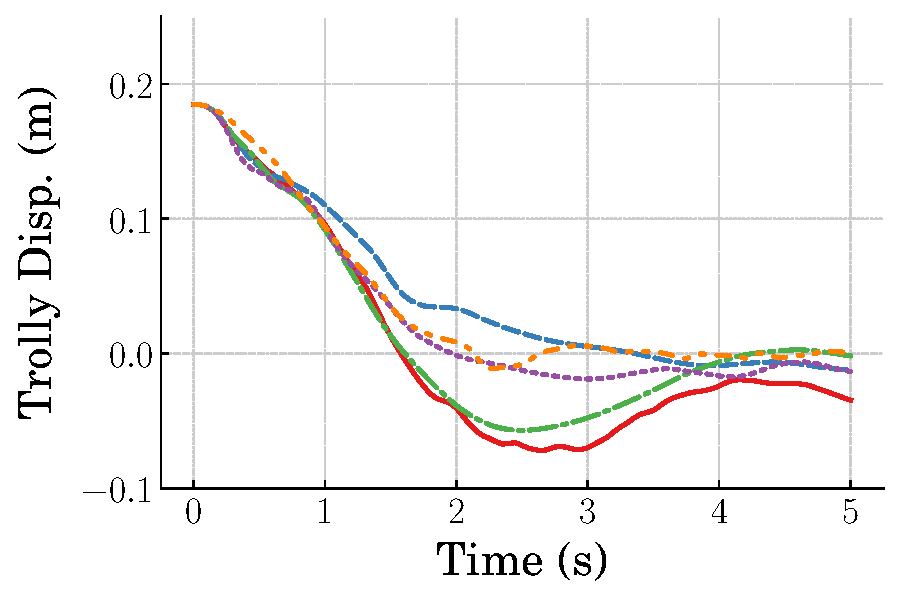
\includegraphics[width=\textwidth]{figures/figures_Interpretability/Mean_ISE_dpcrane_cubic_1_bins/curve_fit_time_responses/RL_PD/agent_0p18_Trolly_Disp.pdf}
        \caption{Agent response}
        \label{subfig_chap5:dpcrane_RL_PD_trolley_0.185_init_agent_unclipped}
    \end{subfigure}
    \hfill
    \begin{subfigure}[b]{0.32\textwidth}
        \centering
        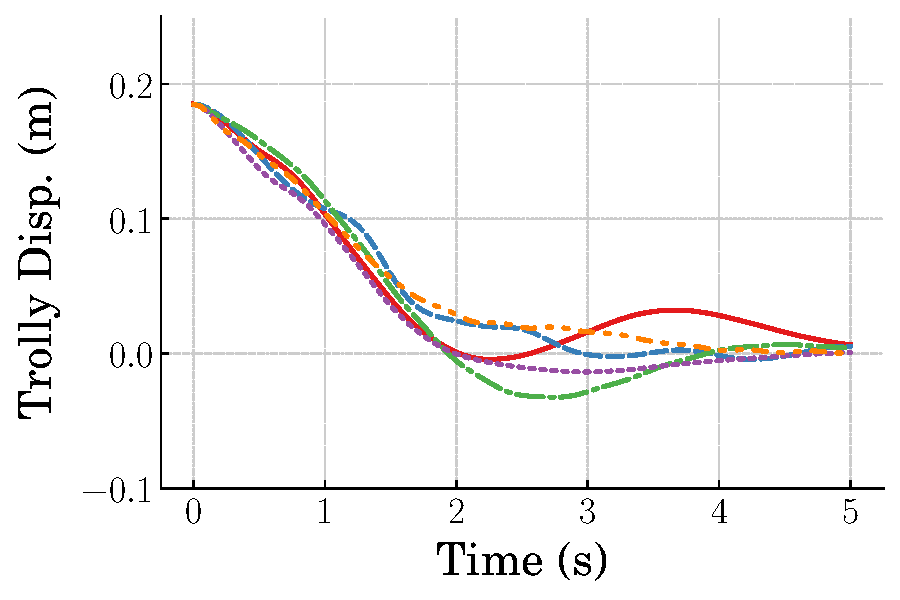
\includegraphics[width=\textwidth]{figures/figures_Interpretability/Mean_ISE_dpcrane_cubic_1_bins/curve_fit_time_responses/RL_PD/curve_fit_0p18_Trolly_Disp.pdf}
        \caption{Curve fit with 1 bin}
        \label{subfig_chap5:dpcrane_RL_PD_trolley_0.185_init_curve_fit_1_bins_unclipped}
    \end{subfigure}
    \hfill
    \begin{subfigure}[b]{0.32\textwidth}
        \centering
        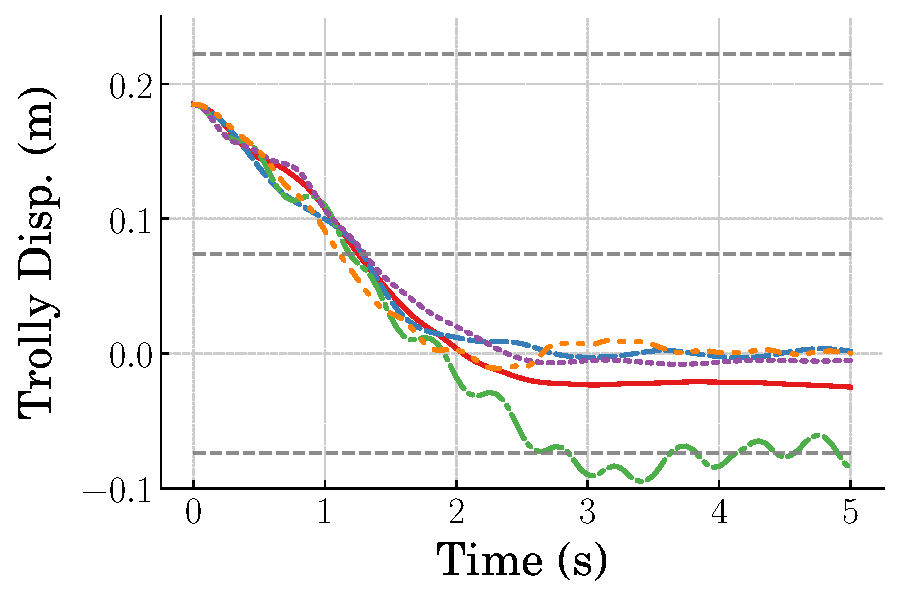
\includegraphics[width=\textwidth]{figures/figures_Interpretability/Mean_ISE_dpcrane_cubic_5_bins/curve_fit_time_responses/RL_PD/curve_fit_0p18_Trolly_Disp.pdf} 
        \caption{Curve fit with 5 bins}
        \label{subfig_chap5:dpcrane_RL_PD_trolley_0.185_init_curve_fit_5_bins_unclipped}
    \end{subfigure}
    \hfill
    \caption{RL-PD curve fit responses for crane trolley for $x(0)=0.185\si{\meter}$}
    \label{fig_chap5:dpcrane_RL_PD_trolley_0.185_init_unclipped}
\end{figure}
%
Figure~\ref{fig_chap5:dpcrane_RL_PD_trolley_0.185_init_unclipped} shows the time responses from the switching controllers for RL-PD. For both the case with one local controller in Figure~\ref{subfig_chap5:dpcrane_RL_PD_trolley_0.185_init_curve_fit_1_bins_unclipped} and the case with five local controllers in Figure~\ref{subfig_chap5:dpcrane_RL_PD_trolley_0.185_init_curve_fit_5_bins_unclipped}, the switching controllers tend to converge close to the desired displacement at $x=0$, similar to the agent controller. However, the response shown in green for the five local controller case does not satisfactorily approximate the corresponding agent response since
it oscillates about the switching boundary indicated by the dashed gray horizontal line.

%
\begin{figure}
    \centering
    \begin{subfigure}[b]{0.32\textwidth}
        \centering
        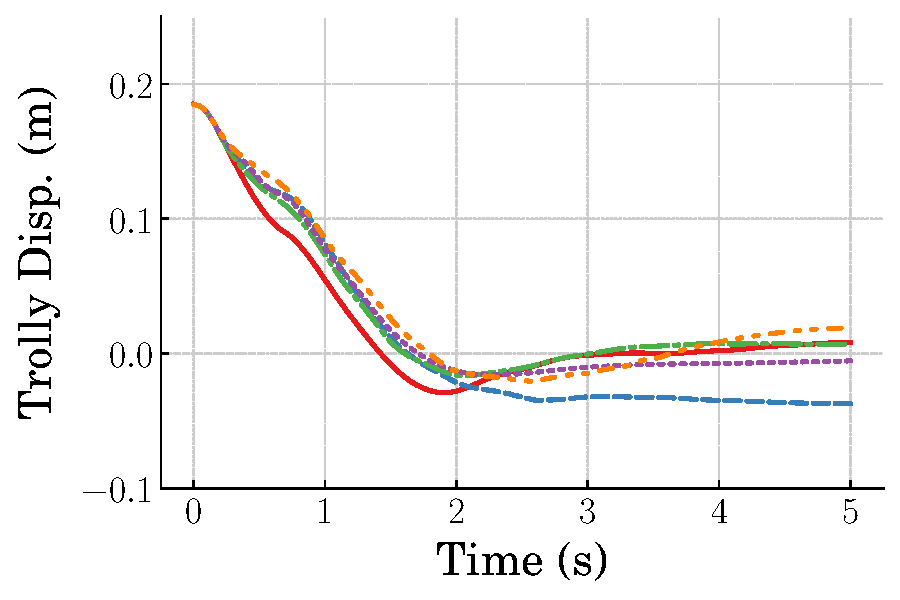
\includegraphics[width=\textwidth]{figures/figures_Interpretability/Mean_ISE_dpcrane_cubic_1_bins/curve_fit_time_responses/RL_LA/agent_0p18_Trolly_Disp.pdf}
        \caption{Agent response}
        \label{subfig_chap5:dpcrane_RL_LA_trolley_0.185_init_agent_unclipped}
    \end{subfigure}
    \hfill
    \begin{subfigure}[b]{0.32\textwidth}
        \centering
        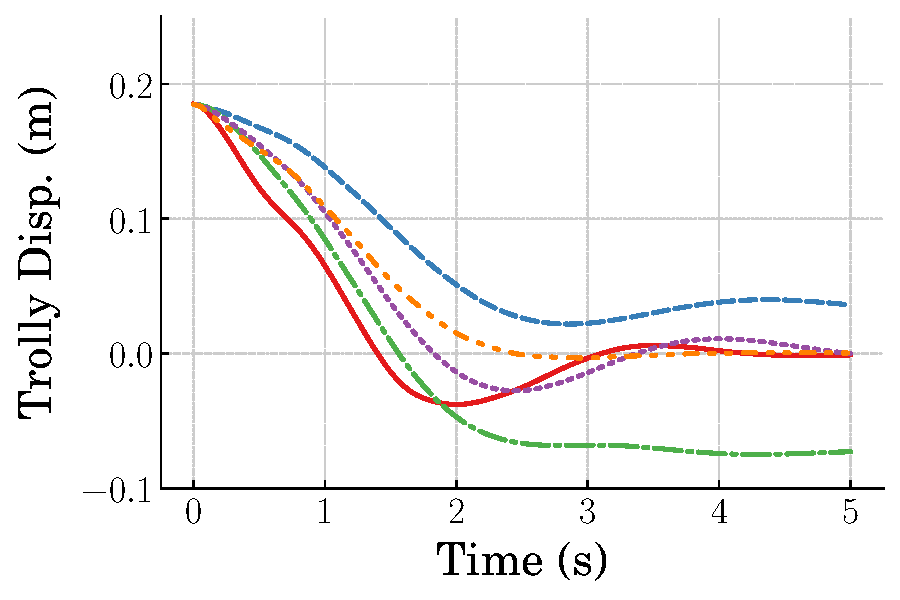
\includegraphics[width=\textwidth]{figures/figures_Interpretability/Mean_ISE_dpcrane_cubic_1_bins/curve_fit_time_responses/RL_LA/curve_fit_0p18_Trolly_Disp.pdf}
        \caption{1 local approximation}
        \label{subfig_chap5:dpcrane_RL_LA_trolley_0.185_init_curve_fit_1_bins_unclipped}
    \end{subfigure}
    \hfill
    \begin{subfigure}[b]{0.32\textwidth}
        \centering
        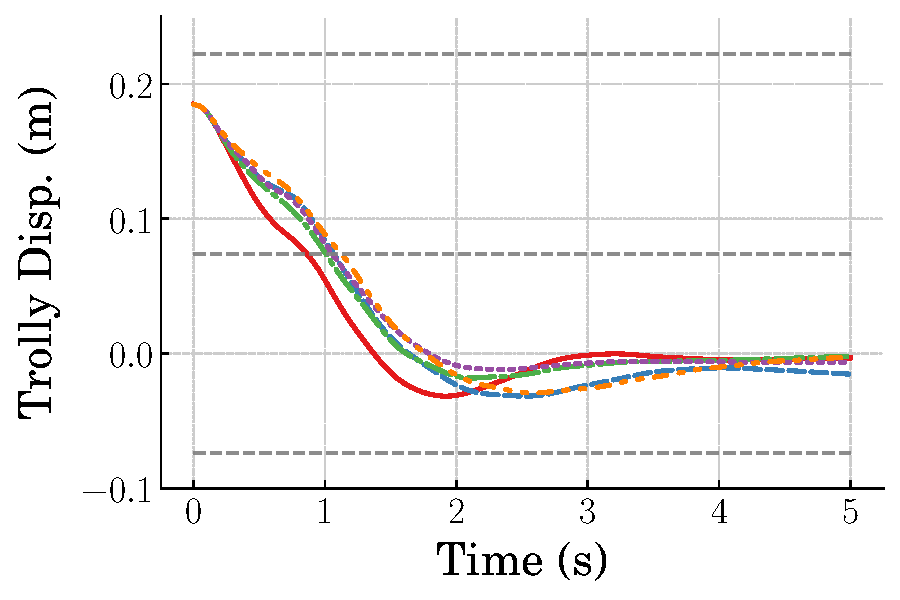
\includegraphics[width=\textwidth]{figures/figures_Interpretability/Mean_ISE_dpcrane_cubic_5_bins/curve_fit_time_responses/RL_LA/curve_fit_0p18_Trolly_Disp.pdf} 
        \caption{5 local approximations}
        \label{subfig_chap5:dpcrane_RL_LA_trolley_0.185_init_curve_fit_5_bins_unclipped}
    \end{subfigure}
    \hfill
    \caption{RL-LA curve fit responses for crane trolley for $x(0)=0.185\si{\meter}$}
    \label{fig_chap5:dpcrane_RL_LA_trolley_0.185_init_unclipped}
\end{figure}
%
The RL-LA time responses for the switching controller approximations are shown in Figure~\ref{fig_chap5:dpcrane_RL_LA_trolley_0.185_init_unclipped}. The agent responses in Figure~\ref{subfig_chap5:dpcrane_RL_LA_trolley_0.185_init_agent_unclipped} show that the trolley responses tend to converge near the desired displacement with only low steady-state error. The approximate controllers with one local controller in Figure~\ref{subfig_chap5:dpcrane_RL_LA_trolley_0.185_init_curve_fit_1_bins_unclipped} have three responses that settle to zero displacement. However, two of the responses have much higher steady-state error than the corresponding agent responses. The responses for the case with five local controllers in Figure~\ref{subfig_chap5:dpcrane_RL_LA_trolley_0.185_init_curve_fit_5_bins_unclipped} tend to converge to zero displacement with less steady-state error than both the agent responses and the one local approximation case.

%
\begin{figure}
    \centering
    \begin{subfigure}[b]{0.32\textwidth}
        \centering
        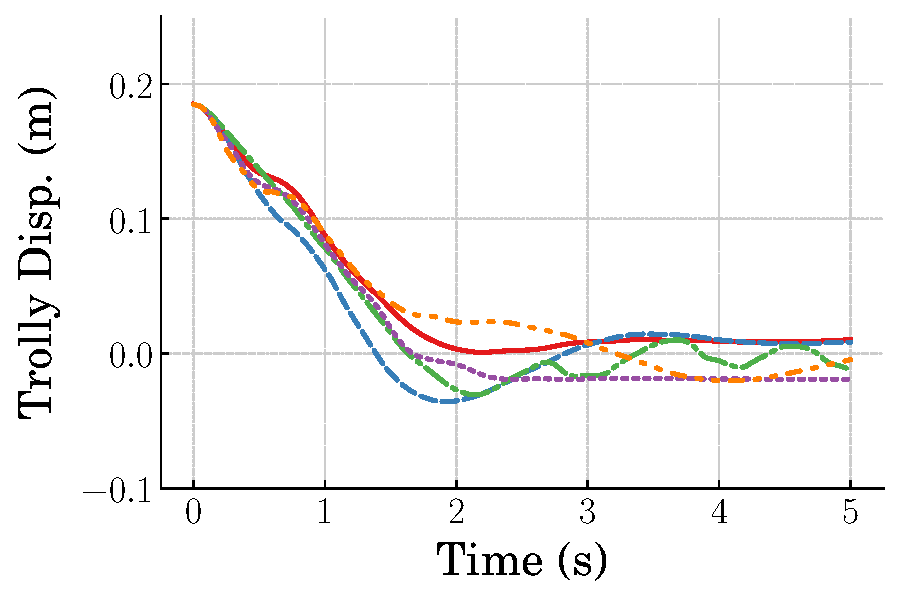
\includegraphics[width=\textwidth]{figures/figures_Interpretability/Mean_ISE_dpcrane_cubic_1_bins/curve_fit_time_responses/RL_PD_LA/agent_0p18_Trolly_Disp.pdf}
        \caption{Agent response}
        \label{subfig_chap5:dpcrane_RL_PD_LA_trolley_0.185_init_agent_unclipped}
    \end{subfigure}
    \hfill
    \begin{subfigure}[b]{0.32\textwidth}
        \centering
        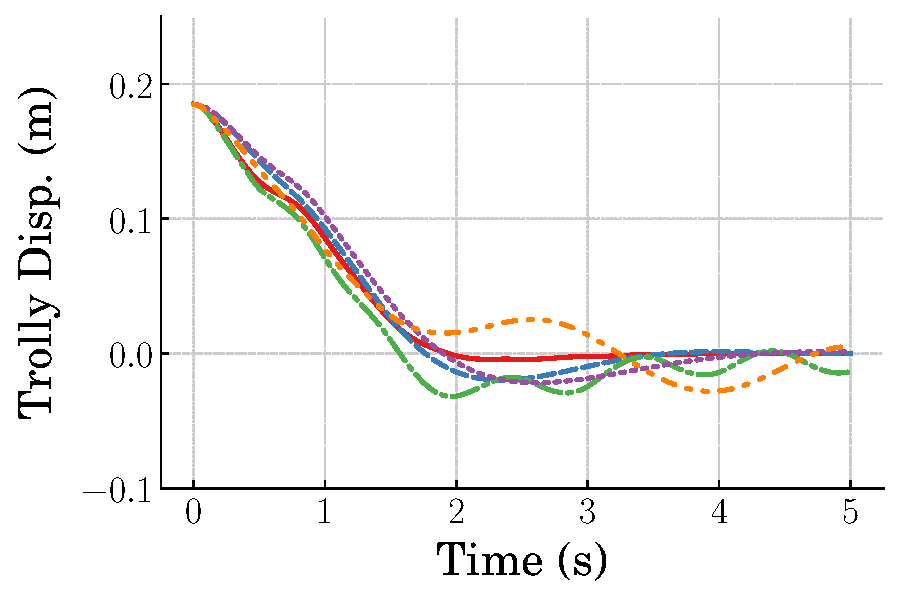
\includegraphics[width=\textwidth]{figures/figures_Interpretability/Mean_ISE_dpcrane_cubic_1_bins/curve_fit_time_responses/RL_PD_LA/curve_fit_0p18_Trolly_Disp.pdf}
        \caption{Curve fit with 1 bin}
        \label{subfig_chap5:dpcrane_RL_PD_LA_trolley_0.185_init_curve_fit_1_bins_unclipped}
    \end{subfigure}
    \hfill
    \begin{subfigure}[b]{0.32\textwidth}
        \centering
        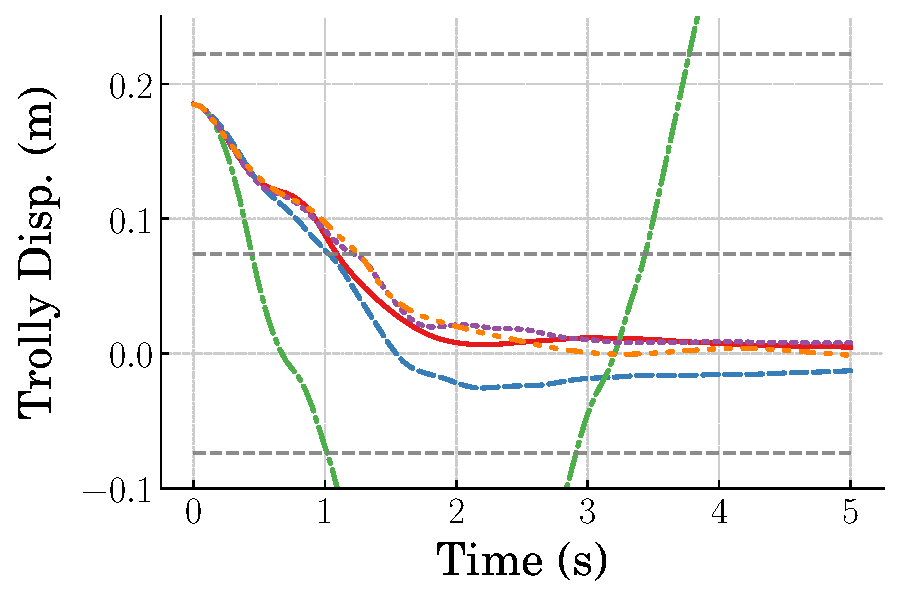
\includegraphics[width=\textwidth]{figures/figures_Interpretability/Mean_ISE_dpcrane_cubic_5_bins/curve_fit_time_responses/RL_PD_LA/curve_fit_0p18_Trolly_Disp.pdf} 
        \caption{Curve fit with 5 bins}
        \label{subfig_chap5:dpcrane_RL_PD_LA_trolley_0.185_init_curve_fit_5_bins_unclipped}
    \end{subfigure}
    \hfill
    \caption{RL-PD-LA curve fit responses for crane trolley for $x(0)=0.185\si{\meter}$}
    \label{fig_chap5:dpcrane_RL_PD_LA_trolley_0.185_init_unclipped}
\end{figure}
%
Figure~\ref{fig_chap5:dpcrane_RL_PD_LA_trolley_0.185_init_unclipped} shows the responses of the switching controllers for RL-PD-LA. Similar to the responses for the other controller types for the crane, the switching controllers tend to satisfactorily approximate the responses of the agent controller by converging near the equilibrium. However, one of the responses for the five local approximation case in Figure~\ref{subfig_chap5:dpcrane_RL_PD_LA_trolley_0.185_init_curve_fit_5_bins_unclipped} is unstable and diverges from the desired displacement.
% \rnotes{It's a bad fit in that subregion. Its response is too fast there. If it starts in the region that contains the equilibrium, it is stable.}

Figure~\ref{fig_chap5:dpcrane_payload_unclipped_approx_error} shows the mean ISE of the payload angular displacements for the switching controllers when the initial displacement of the trolley is $x(0)=0.185\si{\meter}$.
%
% The mean ISE of the payload angular displacements for the switching controllers is shown in Figure~\ref{fig_chap5:dpcrane_payload_unclipped_approx_error}.
The ISE is plotted against the initial displacement of the trolley since that is the scheduling variable. Similar to the ISE of the trolley responses, the controllers using one local approximation of the agents in Figure~\ref{subfig_chap5:dpcrane_payload_unclipped_approx_error_1_bins} have smoother trends than the switching controllers using five local approximations in Figure~\ref{subfig_chap5:dpcrane_payload_unclipped_approx_error_5_bins}. The case with five local approximations has more peaks with higher variance. These peaks are explained by the time responses below.
%
\begin{figure}[t]
    \centering
    \begin{subfigure}[b]{0.49\textwidth}
        \centering
        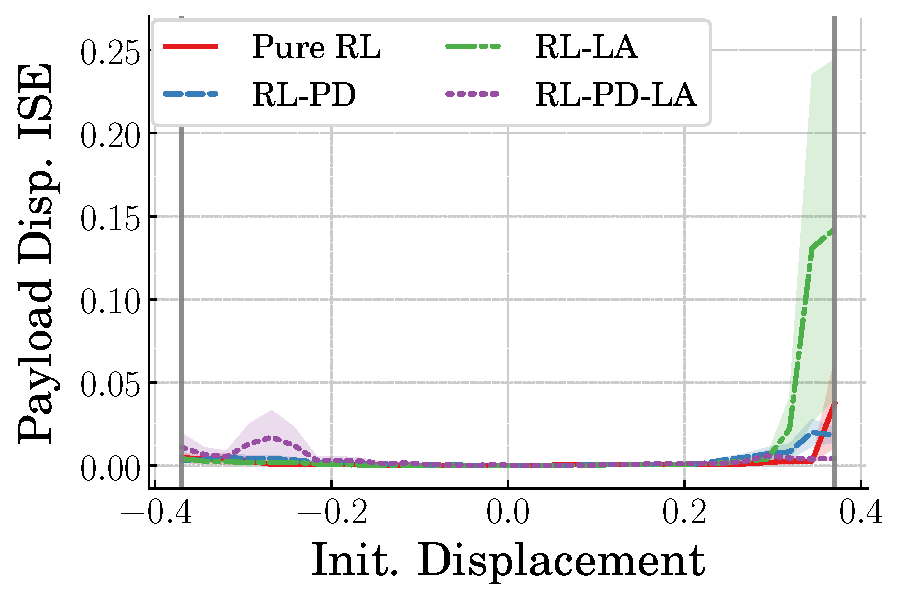
\includegraphics[width=\textwidth]{figures/figures_Interpretability/Mean_ISE_dpcrane_cubic_1_bins/Mean_ISE_dpcrane_cubic_Payload_Disp_1_bins.pdf}
        \caption{1 local approximation}
        \label{subfig_chap5:dpcrane_payload_unclipped_approx_error_1_bins}
    \end{subfigure}
    \hfill
    \begin{subfigure}[b]{0.49\textwidth}
        \centering
        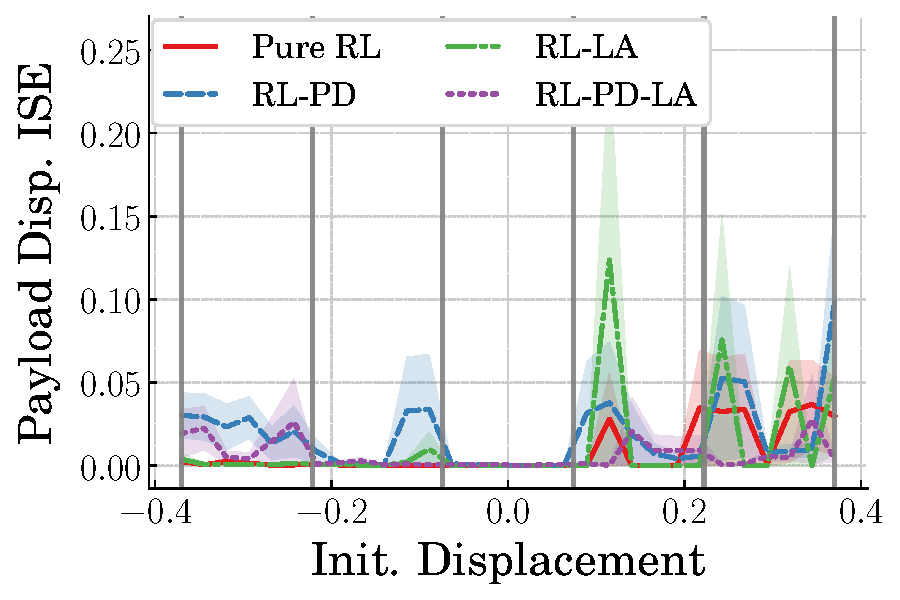
\includegraphics[width=\textwidth]{figures/figures_Interpretability/Mean_ISE_dpcrane_cubic_5_bins/Mean_ISE_dpcrane_cubic_Payload_Disp_5_bins.pdf}
        \caption{5 local approximations}
        \label{subfig_chap5:dpcrane_payload_unclipped_approx_error_5_bins}
    \end{subfigure}
       \caption{ISE of crane payload for local controllers}
       \label{fig_chap5:dpcrane_payload_unclipped_approx_error}
\end{figure}
%

The figures below show the payload time responses for trolley initial displacements of $x(0)=0.185\si{\meter}$. These responses resulted from the same switching controllers shown previously.
%
Figure~\ref{fig_chap5:dpcrane_pure_RL_payload_0.185_init_unclipped} shows the payload time responses of the switching controllers for Pure RL.
% The payload time responses of the switching controllers approximating the Pure RL controllers are shown in Figure~\ref{fig_chap5:dpcrane_pure_RL_payload_0.185_init_unclipped}.
The crane started at rest with an initial trolley displacement of $x=0.185\si{\meter}$ and pendulum angular displacements of $\theta_1=\theta_2=0$. The pendulum responses with the switching controllers were able to maintain low oscillation amplitude and closely approximate the agent responses. The responses with one local approximation in Figure~\ref{subfig_chap5:dpcrane_pure_RL_payload_0.185_init_curve_fit_1_bins_unclipped} have a lower peak magnitude than the responses with five local approximations in Figure~\ref{subfig_chap5:dpcrane_pure_RL_payload_0.185_init_curve_fit_5_bins_unclipped}. However, the higher peak amplitude with five local approximations more closely matches that of the agent response in Figure~\ref{subfig_chap5:dpcrane_pure_RL_payload_0.185_init_agent_unclipped}.
%
\begin{figure}
    \centering
    \begin{subfigure}[b]{0.32\textwidth}
        \centering
        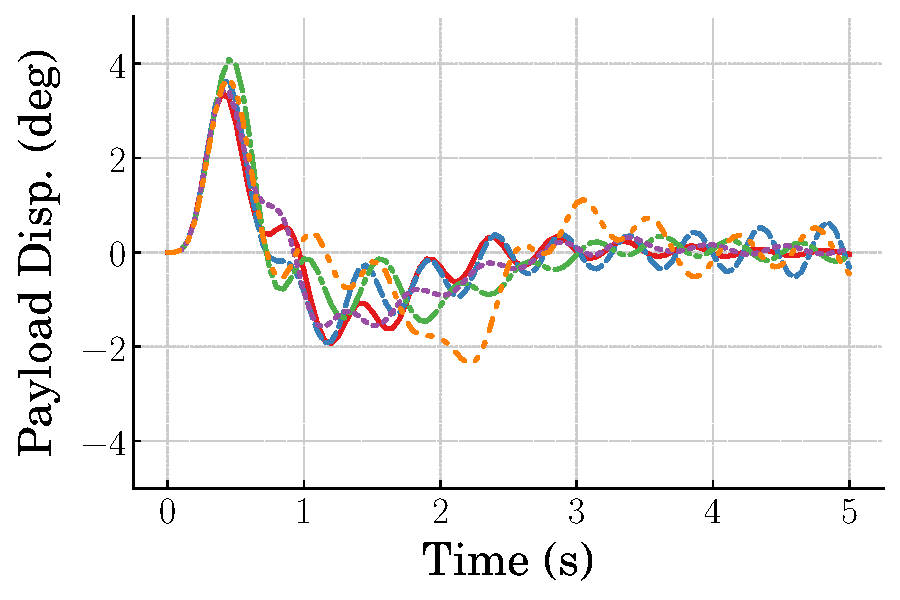
\includegraphics[width=\textwidth]{figures/figures_Interpretability/Mean_ISE_dpcrane_cubic_1_bins/curve_fit_time_responses/pure_RL/agent_0p18_Payload_Disp.pdf}
        \caption{Agent response}
        \label{subfig_chap5:dpcrane_pure_RL_payload_0.185_init_agent_unclipped}
    \end{subfigure}
    \hfill
    \begin{subfigure}[b]{0.32\textwidth}
        \centering
        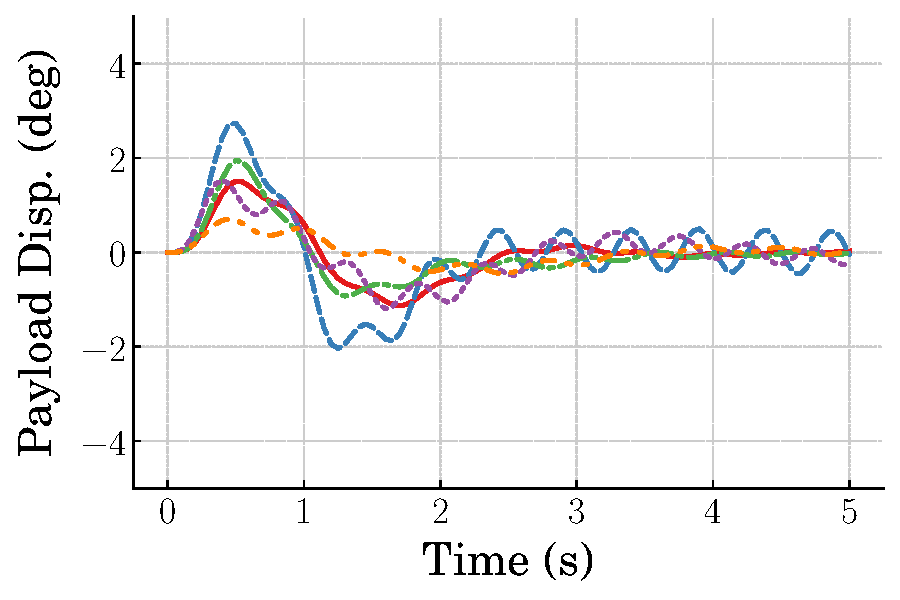
\includegraphics[width=\textwidth]{figures/figures_Interpretability/Mean_ISE_dpcrane_cubic_1_bins/curve_fit_time_responses/pure_RL/curve_fit_0p18_Payload_Disp.pdf}
        \caption{1 local approximation}
        \label{subfig_chap5:dpcrane_pure_RL_payload_0.185_init_curve_fit_1_bins_unclipped}
    \end{subfigure}
    \hfill
    \begin{subfigure}[b]{0.32\textwidth}
        \centering
        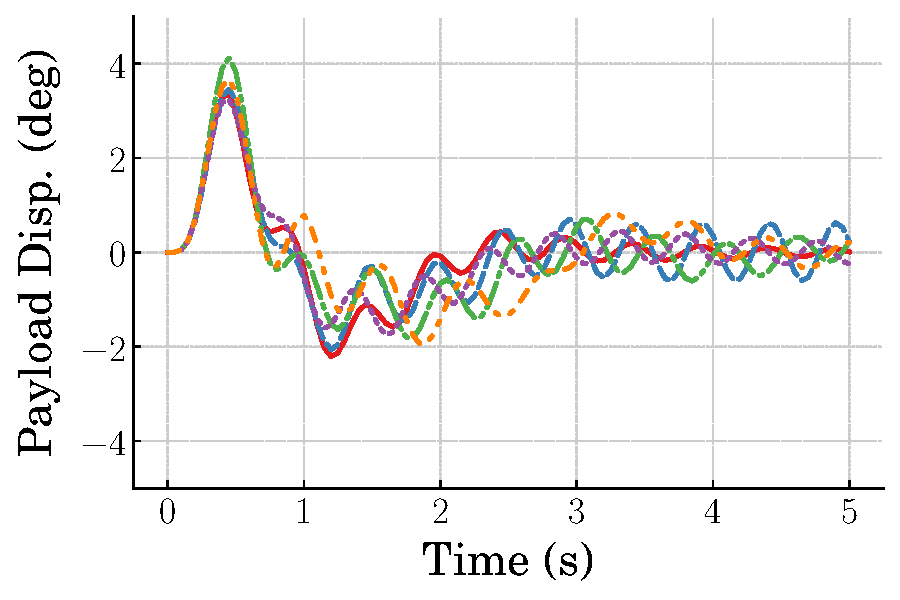
\includegraphics[width=\textwidth]{figures/figures_Interpretability/Mean_ISE_dpcrane_cubic_5_bins/curve_fit_time_responses/pure_RL/curve_fit_0p18_Payload_Disp.pdf} 
        \caption{5 local approximations}
        \label{subfig_chap5:dpcrane_pure_RL_payload_0.185_init_curve_fit_5_bins_unclipped}
    \end{subfigure}
    \hfill
    \caption{Pure RL curve fit responses for crane payload for $x(0)=0.185\si{\meter}$}
    \label{fig_chap5:dpcrane_pure_RL_payload_0.185_init_unclipped}
\end{figure}
%

The time responses for the RL-PD switching controllers are in Figure~\ref{fig_chap5:dpcrane_RL_PD_payload_0.185_init_unclipped}. Most of the responses have low oscillation amplitude and reasonably match the agent responses in Figure~\ref{subfig_chap5:dpcrane_RL_PD_payload_0.185_init_agent_unclipped}; however, the response shown in green for five local approximations in Figure~\ref{subfig_chap5:dpcrane_RL_PD_payload_0.185_init_curve_fit_5_bins_unclipped} has significantly higher oscillation amplitude. This corresponds to the trolley response in Figure~\ref{subfig_chap5:dpcrane_RL_PD_trolley_0.185_init_curve_fit_5_bins_unclipped} that oscillated about the switching boundary.
%
\begin{figure}
    \centering
    \begin{subfigure}[b]{0.32\textwidth}
        \centering
        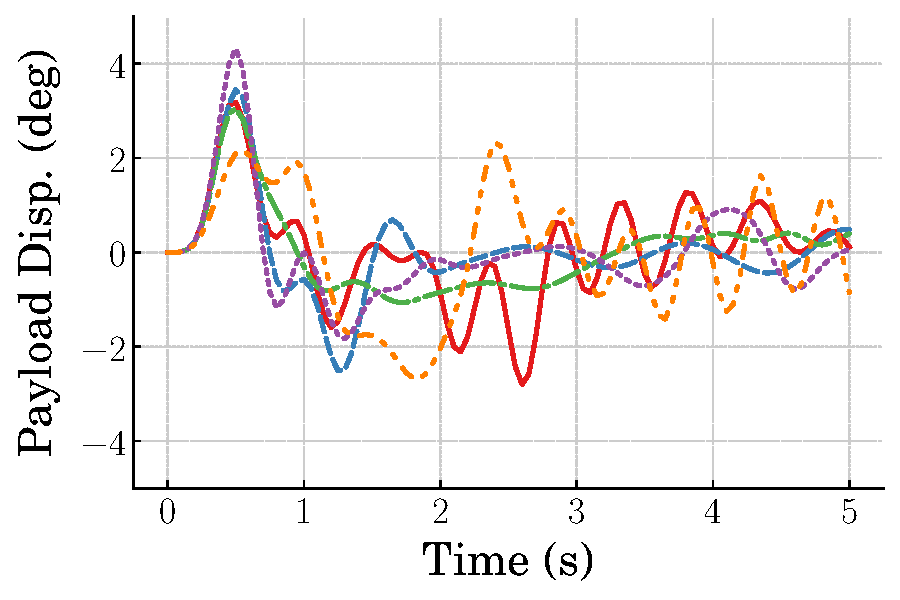
\includegraphics[width=\textwidth]{figures/figures_Interpretability/Mean_ISE_dpcrane_cubic_1_bins/curve_fit_time_responses/RL_PD/agent_0p18_Payload_Disp.pdf}
        \caption{Agent response}
        \label{subfig_chap5:dpcrane_RL_PD_payload_0.185_init_agent_unclipped}
    \end{subfigure}
    \hfill
    \begin{subfigure}[b]{0.32\textwidth}
        \centering
        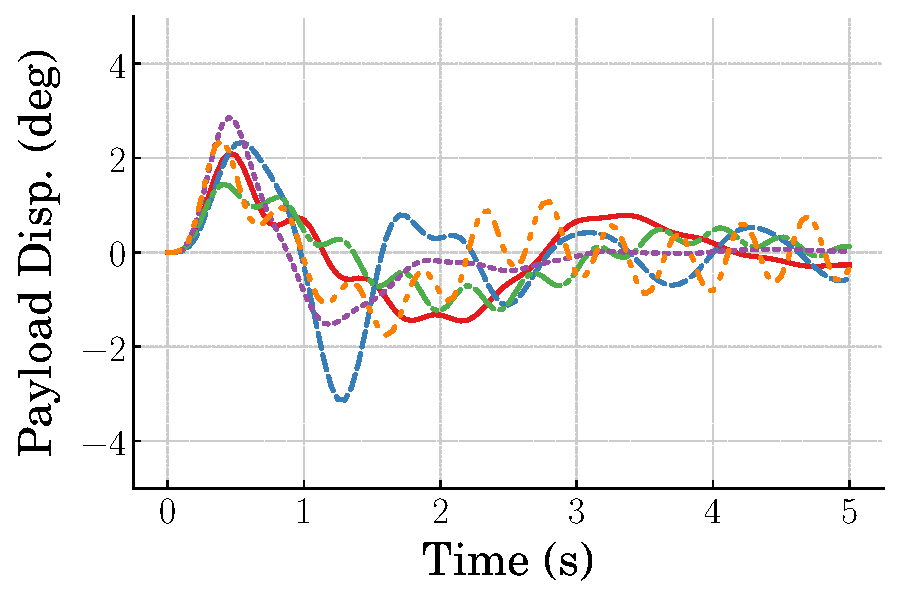
\includegraphics[width=\textwidth]{figures/figures_Interpretability/Mean_ISE_dpcrane_cubic_1_bins/curve_fit_time_responses/RL_PD/curve_fit_0p18_Payload_Disp.pdf}
        \caption{1 local approximation}
        \label{subfig_chap5:dpcrane_RL_PD_payload_0.185_init_curve_fit_1_bins_unclipped}
    \end{subfigure}
    \hfill
    \begin{subfigure}[b]{0.32\textwidth}
        \centering
        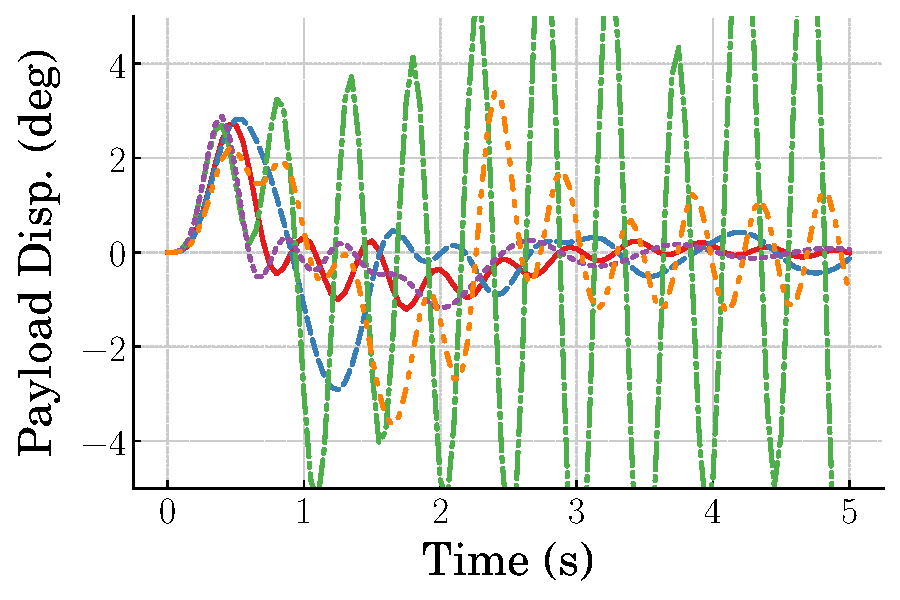
\includegraphics[width=\textwidth]{figures/figures_Interpretability/Mean_ISE_dpcrane_cubic_5_bins/curve_fit_time_responses/RL_PD/curve_fit_0p18_Payload_Disp.pdf} 
        \caption{5 local approximation}
        \label{subfig_chap5:dpcrane_RL_PD_payload_0.185_init_curve_fit_5_bins_unclipped}
    \end{subfigure}
    \hfill
    \caption{RL-PD curve fit responses for crane payload for $x(0)=0.185\si{\meter}$}
    \label{fig_chap5:dpcrane_RL_PD_payload_0.185_init_unclipped}
\end{figure}
%

The payload responses of the switched controllers for RL-LA are shown in Figure~\ref{fig_chap5:dpcrane_RL_LA_payload_0.185_init_unclipped}.
The cases with one local approximation in Figure~\ref{subfig_chap5:dpcrane_RL_LA_payload_0.185_init_curve_fit_1_bins_unclipped} and five local approximations in Figure~\ref{subfig_chap5:dpcrane_RL_LA_payload_0.185_init_curve_fit_5_bins_unclipped} both satisfactorily match the agent responses by mitigating oscillation. However, the case with five local controllers more closely matches the agent responses.
% \rph{Both the one local approximation controller and the five local approximation controller in satisfactorily match the agent responses. The responses of the five local approximation controller more closely match the responses of the agent.}
%
\begin{figure}
    \centering
    \begin{subfigure}[b]{0.32\textwidth}
        \centering
        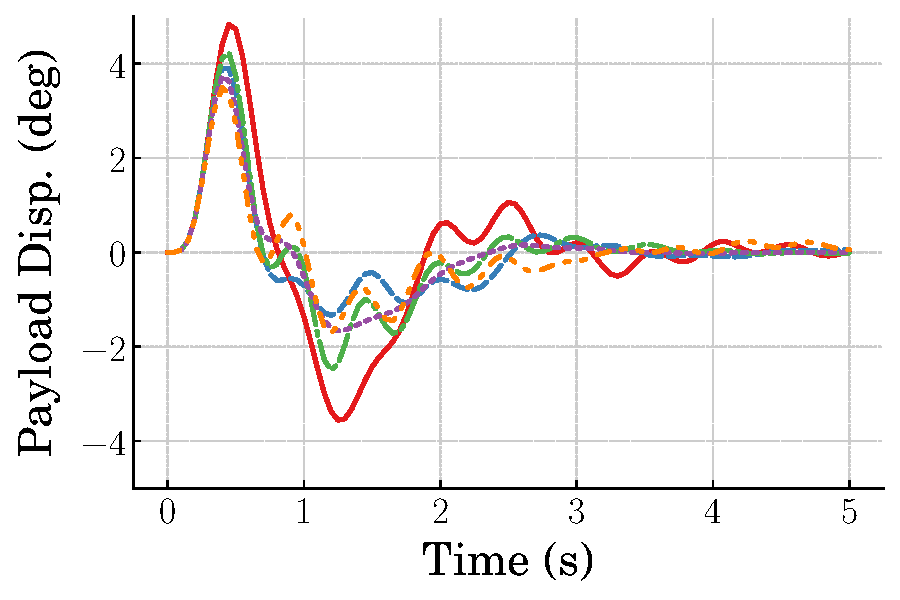
\includegraphics[width=\textwidth]{figures/figures_Interpretability/Mean_ISE_dpcrane_cubic_1_bins/curve_fit_time_responses/RL_LA/agent_0p18_Payload_Disp.pdf}
        \caption{Agent response}
        \label{subfig_chap5:dpcrane_RL_LA_payload_0.185_init_agent_unclipped}
    \end{subfigure}
    \hfill
    \begin{subfigure}[b]{0.32\textwidth}
        \centering
        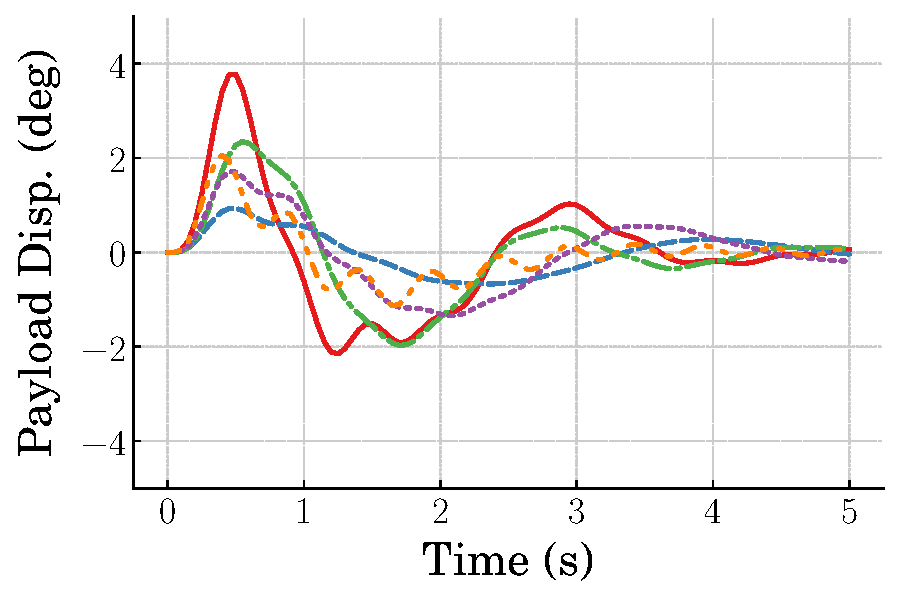
\includegraphics[width=\textwidth]{figures/figures_Interpretability/Mean_ISE_dpcrane_cubic_1_bins/curve_fit_time_responses/RL_LA/curve_fit_0p18_Payload_Disp.pdf}
        \caption{1 local approximation}
        \label{subfig_chap5:dpcrane_RL_LA_payload_0.185_init_curve_fit_1_bins_unclipped}
    \end{subfigure}
    \hfill
    \begin{subfigure}[b]{0.32\textwidth}
        \centering
        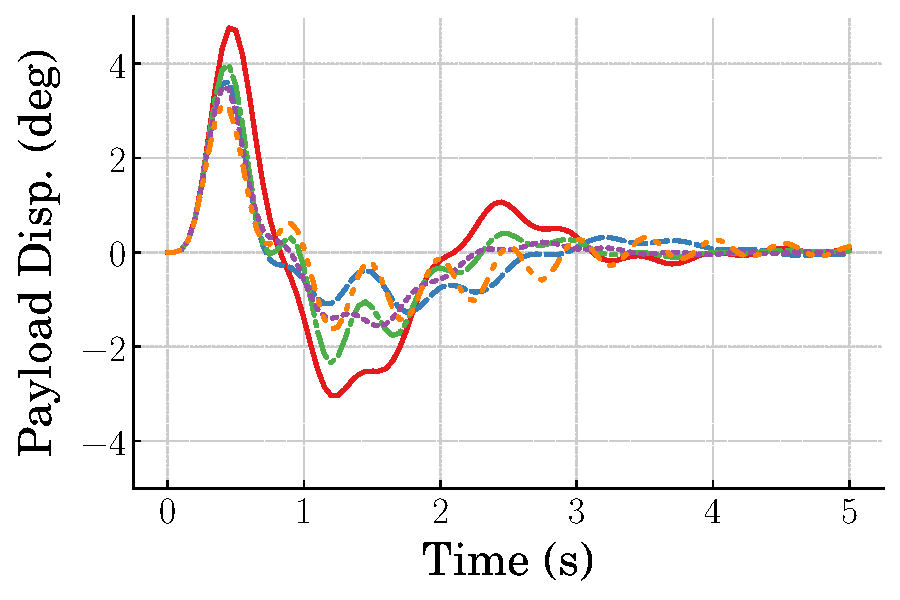
\includegraphics[width=\textwidth]{figures/figures_Interpretability/Mean_ISE_dpcrane_cubic_5_bins/curve_fit_time_responses/RL_LA/curve_fit_0p18_Payload_Disp.pdf} 
        \caption{5 local approximations}
        \label{subfig_chap5:dpcrane_RL_LA_payload_0.185_init_curve_fit_5_bins_unclipped}
    \end{subfigure}
    \hfill
    \caption{RL-LA curve fit responses for crane payload for $x(0)=0.185\si{\meter}$}
    \label{fig_chap5:dpcrane_RL_LA_payload_0.185_init_unclipped}
\end{figure}
%

Figure~\ref{fig_chap5:dpcrane_RL_PD_LA_payload_0.185_init_unclipped} shows the time responses of the switching controllers approximating the RL-PD-LA agents. The approximations tend to satisfactorily match the responses of the agents. However, the response shown in orange for the case with one local approximation in Figure~\ref{subfig_chap5:dpcrane_RL_PD_LA_payload_0.185_init_curve_fit_1_bins_unclipped} has higher oscillation amplitude than the corresponding agent responses. Also, one of the responses with five local approximations in Figure~\ref{subfig_chap5:dpcrane_RL_PD_LA_payload_0.185_init_curve_fit_5_bins_unclipped} has significantly more payload oscillation amplitude than the agent responses. The other responses in this case quickly mitigate the residual oscillation.
%
\begin{figure}
    \centering
    \begin{subfigure}[b]{0.32\textwidth}
        \centering
        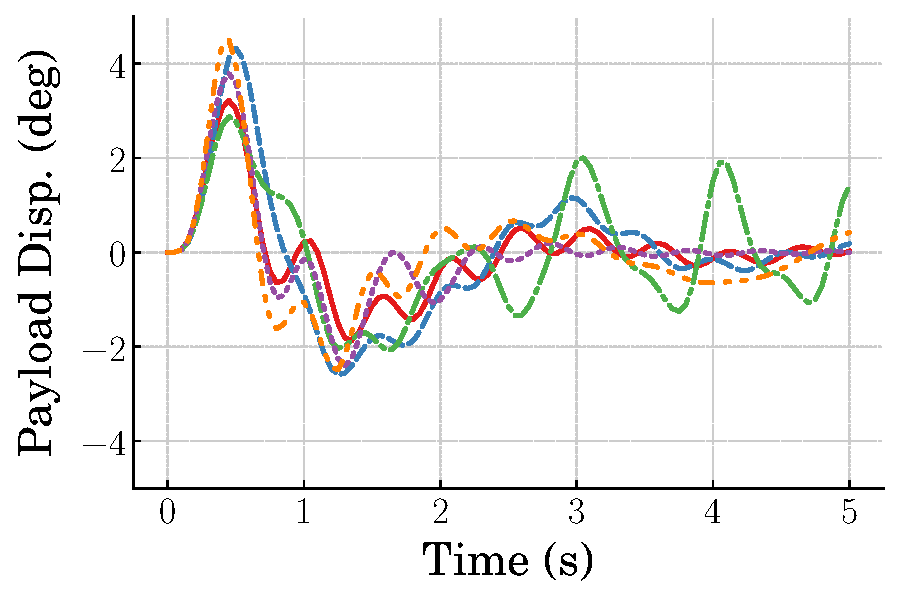
\includegraphics[width=\textwidth]{figures/figures_Interpretability/Mean_ISE_dpcrane_cubic_1_bins/curve_fit_time_responses/RL_PD_LA/agent_0p18_Payload_Disp.pdf}
        \caption{Agent response}
        \label{subfig_chap5:dpcrane_RL_PD_LA_payload_0.185_init_agent_unclipped}
    \end{subfigure}
    \hfill
    \begin{subfigure}[b]{0.32\textwidth}
        \centering
        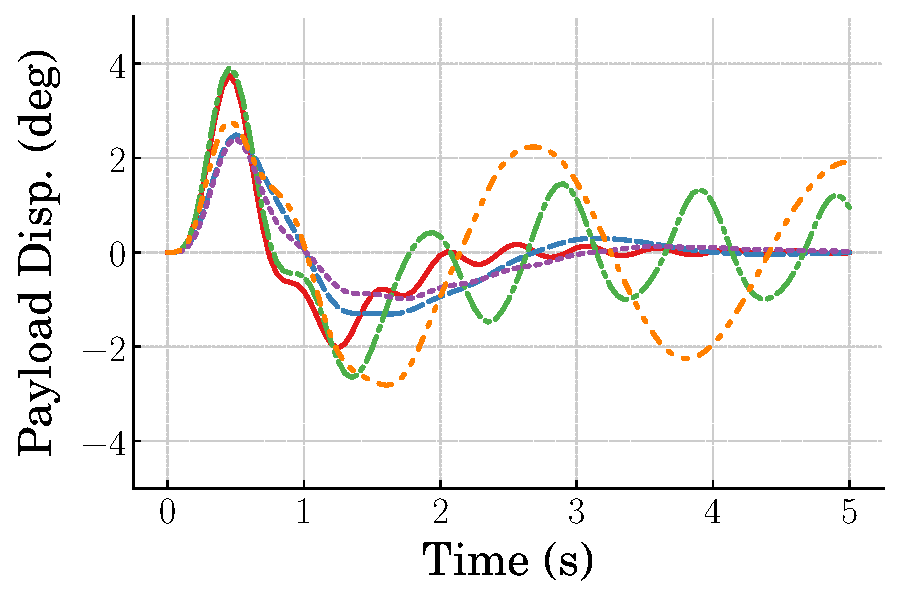
\includegraphics[width=\textwidth]{figures/figures_Interpretability/Mean_ISE_dpcrane_cubic_1_bins/curve_fit_time_responses/RL_PD_LA/curve_fit_0p18_Payload_Disp.pdf}
        \caption{1 local approximation}
        \label{subfig_chap5:dpcrane_RL_PD_LA_payload_0.185_init_curve_fit_1_bins_unclipped}
    \end{subfigure}
    \hfill
    \begin{subfigure}[b]{0.32\textwidth}
        \centering
        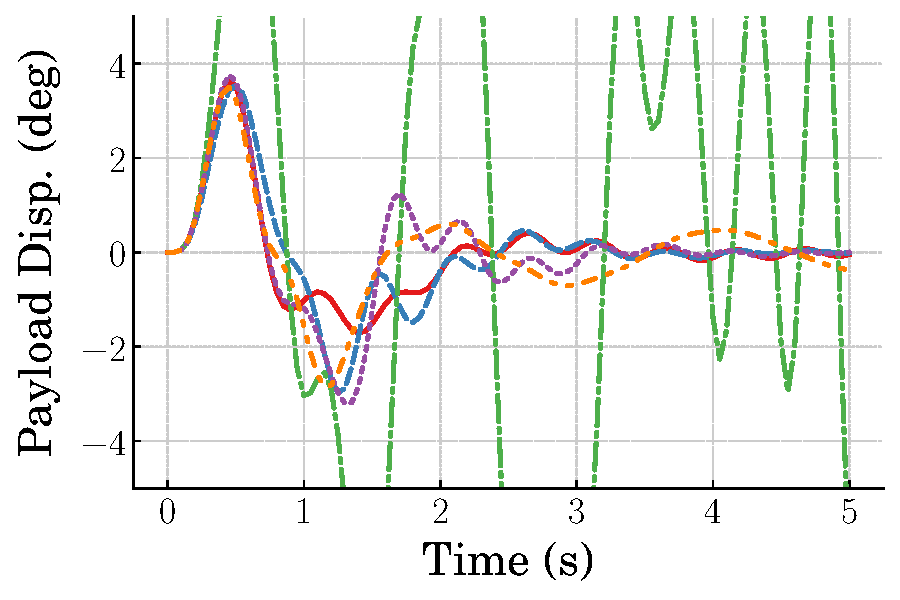
\includegraphics[width=\textwidth]{figures/figures_Interpretability/Mean_ISE_dpcrane_cubic_5_bins/curve_fit_time_responses/RL_PD_LA/curve_fit_0p18_Payload_Disp.pdf} 
        \caption{5 local approximations}
        \label{subfig_chap5:dpcrane_RL_PD_LA_payload_0.185_init_curve_fit_5_bins_unclipped}
    \end{subfigure}
    \hfill
    \caption{RL-PD-LA curve fit responses for crane payload for $x(0)=0.185\si{\meter}$}
    \label{fig_chap5:dpcrane_RL_PD_LA_payload_0.185_init_unclipped}
\end{figure}
%

In general, the switching controller approximations for the double-pendulum crane tend to be able to accurately model the behavior of the agents. Using a larger number of local approximations in the switching controller tended to improve the modeling accuracy between the approximations and the agents.
However, the increase in the number of local approximations also increased the probability for some switching controller responses to be unstable.
% \rph{However, the increase in local approximations also increased the opportunities for some switching controller responses to have significant error from the corresponding agent.}
This instability is common in switching controllers, often caused by discontinuity at the boundary between the local controllers~\cite{Liberzon:1999a,Liberzon:2003a}. This was particularly common for the approximations of controllers that had an agent-driven gain scheduling component. Despite this, the approximations can be used to improve interpretability of the agents by aiding in the development of intuitive understanding of the agent.

\subsection{Inverted Pendulum Agent Approximation}
The same process used to curve fit switching controllers for the double-pendulum crane was repeated for the inverted pendulum controllers:
%
\begin{align*}
&\qquad\qquad\text{Pure RL:} & u&=a_t \qquad\\
&\qquad\qquad\text{RL-LQR:} & u&= -k_1\theta - k_2\dot{\theta} + a_t \qquad\\
%
&\qquad\qquad\text{S-RL-LQR:} & u&= 
\left\{
    \begin{array}{cl}
        % -k_1\theta - k_2\dot{\theta}, & \quad \text{if } -45^\circ \leq \theta \leq 45^\circ\\
        -k_1\theta - k_2\dot{\theta}, & \quad \forall (\theta, \dot{\theta}) \in S_{st}\\
        % a_t, & \quad \text{if else} 
        a_t, & \quad \forall(\theta,\dot{\theta})\notin S_{st}
    \end{array}
    \right. \qquad
\end{align*}
%
where Pure RL is the controller that only uses the agent action as the output, RL-LQR uses LQR as a fixed-gain component as well as a single lumped action, and S-RL-LQR switches between the agent and LQR when the system is near the upright equilibrium.
% \rph{To avoid confusion, the combined controller that switches between RL and LQR will only be referred to as S-RL-LQR, while the approximated controllers will be referred to as switching controller.}
Polynomials were used to generate local approximations as before, where each controller has the form:
% Polynomials are a useful method for general local function approximation~\pc.
%
\begin{equation}
\hat{a}_l=\sum_{i=1}^p a_ix^i + b_i\dot{x}^i + c_i\theta^i + d_i\dot{\theta}^i
\label{eq_chap5:inv_pend_unsat_approx_func}
\end{equation}
%
where $x$ and $\dot{x}$ are the displacement and velocity of the cart, $\theta$ and $\dot{\theta}$ are angular displacement and angular velocity, and $p=3$ is the degree of the polynomial fit. Angular displacement was used as the scheduling variable.
% The degree of the local polynomial necessary to generate an accurate fit is an indication of the complexity of the agent in the local subregion.

\begin{figure}
     \centering
     \begin{subfigure}[b]{0.49\textwidth}
         \centering
         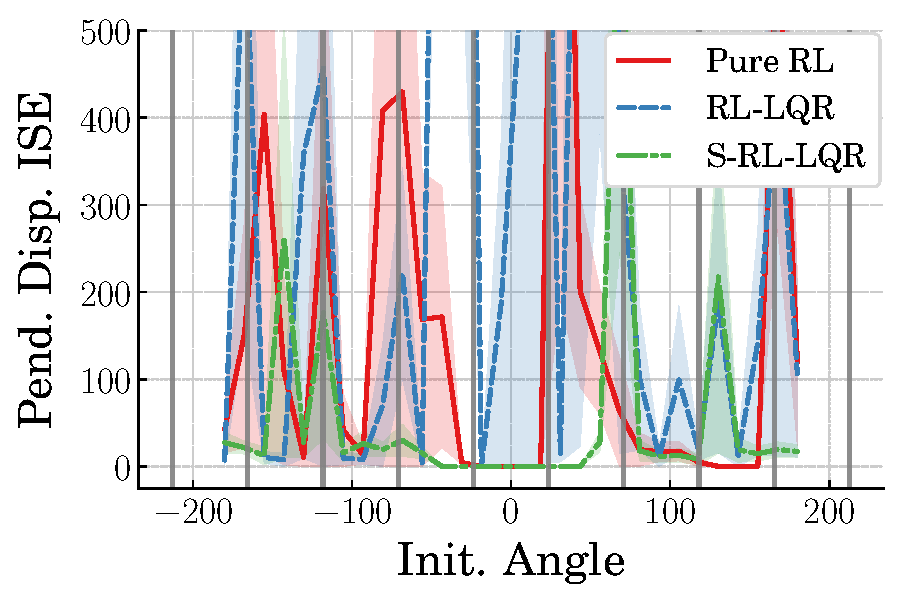
\includegraphics[width=\textwidth]{figures/figures_Interpretability/Mean_ISE_Inverted_Pendulum-v0_cubic_9_bins/Mean_ISE_Inverted_Pendulum-v0_cubic_Pend_Disp_9_bins}
         \caption{9 local approximations}
         \label{subfig_chap5:inv_pend_angle_unclipped_approx_error_9_bins}
     \end{subfigure}
     \hfill
     \begin{subfigure}[b]{0.49\textwidth}
         \centering
         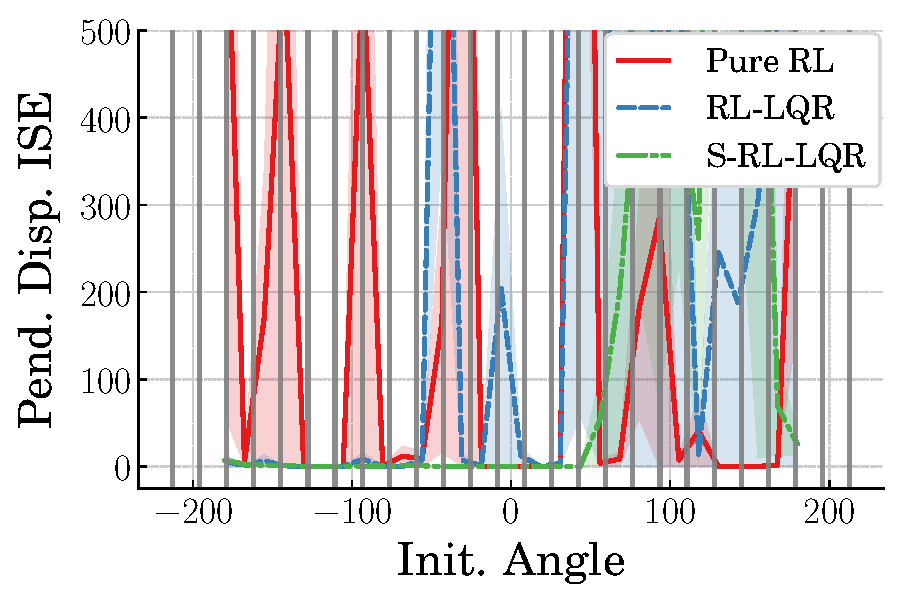
\includegraphics[width=\textwidth]{figures/figures_Interpretability/Mean_ISE_Inverted_Pendulum-v0_cubic_25_bins/Mean_ISE_Inverted_Pendulum-v0_cubic_Pend_Disp_25_bins}
         \caption{25 local approximations}
         \label{subfig_chap5:inv_pend_angle_unclipped_approx_error_25_bins}
     \end{subfigure}
        \caption{ISE of inverted pendulum local controllers for $\theta(0)=180^\circ$}
        \label{fig_chap5:inv_pend_angle_unclipped_approx_error}
\end{figure}

\subsubsection{Approximation for Swing-Up Phase}

Figure~\ref{fig_chap5:inv_pend_angle_unclipped_approx_error} shows the mean ISE of angular displacement between the responses of each agent for each controller type and the corresponding switching controller response. The shaded region shows the standard deviation for each controller type. The ISE was evaluated for a range of initial angular displacements from $\theta=-180^\circ$ to $\theta = 180^\circ$.
%
Figure~\ref{subfig_chap5:inv_pend_angle_unclipped_approx_error_9_bins} shows the mean ISE when the agent is divided into nine local controllers, and Figure~\ref{subfig_chap5:inv_pend_angle_unclipped_approx_error_25_bins} shows the mean ISE for twenty-five local controllers. The boundaries for the local controllers are indicated by the solid vertical gray lines.
Although there are some areas where the mean ISE is low for both the switching controllers with nine local approximations and 25 local approximations, there are many areas with high mean and high standard deviation.
% \rph{The mean ISE is high for most of the range shown in both figures.}
% \rph{The plotting window in the figure is constrained to emphasize the areas where the ISE is lower.}
%
% The plots show significant ISE from most of the initial displacements.
% The sudden spikes in ISE tend to coincide with high standard deviation.
The widest ranges for which ISE is low for Pure RL and S-RL-LQR are found for initial angular displacements near $\theta=0$. The response error for S-RL-LQR is zero for initial angular displacements $-45^\circ<\theta<45^\circ$ due to the agent output being unused in that range.
%
% \rph{The ISE plots shown that the peak error from the RL-LQR approximations tend to be higher than the other controllers and the ISE often exceed the plotting window.}
%
% The ISE plots show that the curve fits for RL-LQR tend to result in more error than for the other controller types.

\begin{figure}
    \centering
    \begin{subfigure}[b]{0.32\textwidth}
        \centering
        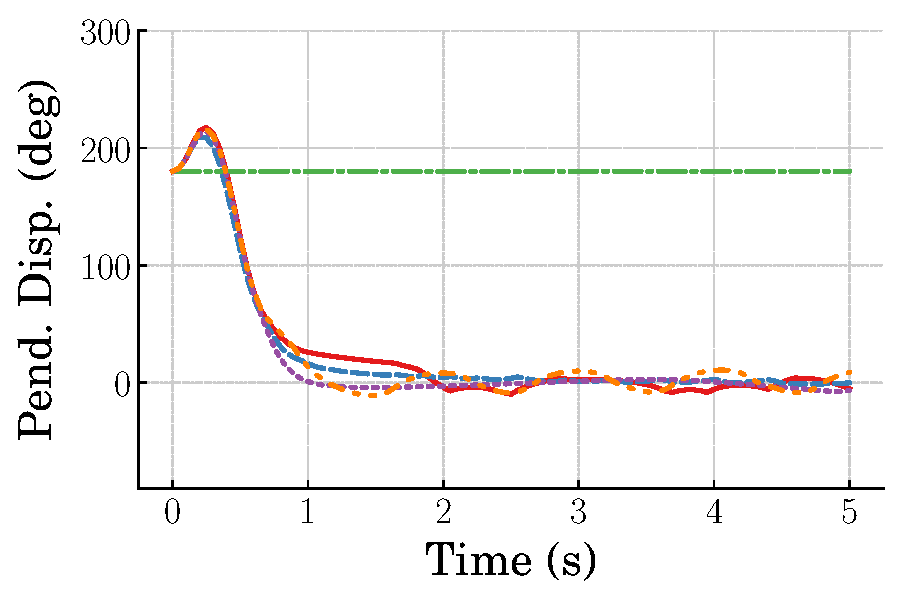
\includegraphics[width=\textwidth]{figures/figures_Interpretability/Mean_ISE_Inverted_Pendulum-v0_cubic_9_bins/Curve_fit_time_responses/pure_RL/agent_Pend_Disp_180.pdf}
        \caption{Agent response}
        \label{subfig_chap5:inv_pend_pure_RL_180_init_agent_unclipped}
    \end{subfigure}
    \hfill
    \begin{subfigure}[b]{0.32\textwidth}
        \centering
        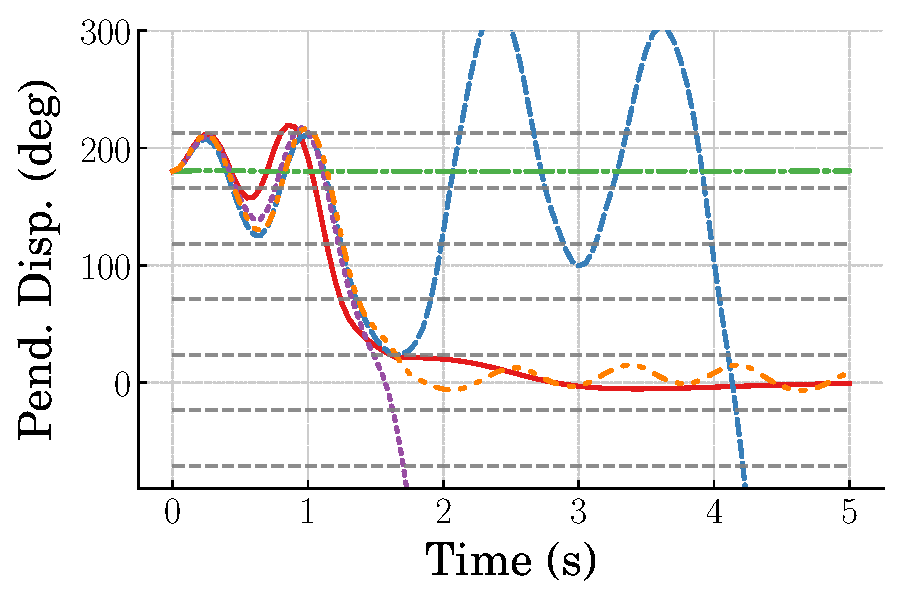
\includegraphics[width=\textwidth]{figures/figures_Interpretability/Mean_ISE_Inverted_Pendulum-v0_cubic_9_bins/Curve_fit_time_responses/pure_RL/curve_fit_Pend_Disp_180.pdf}
        \caption{Curve fit with 9 bins}
        \label{subfig_chap5:inv_pend_pure_RL_180_init_curve_fit_9_bins_unclipped}
    \end{subfigure}
    \hfill
    \begin{subfigure}[b]{0.32\textwidth}
        \centering
        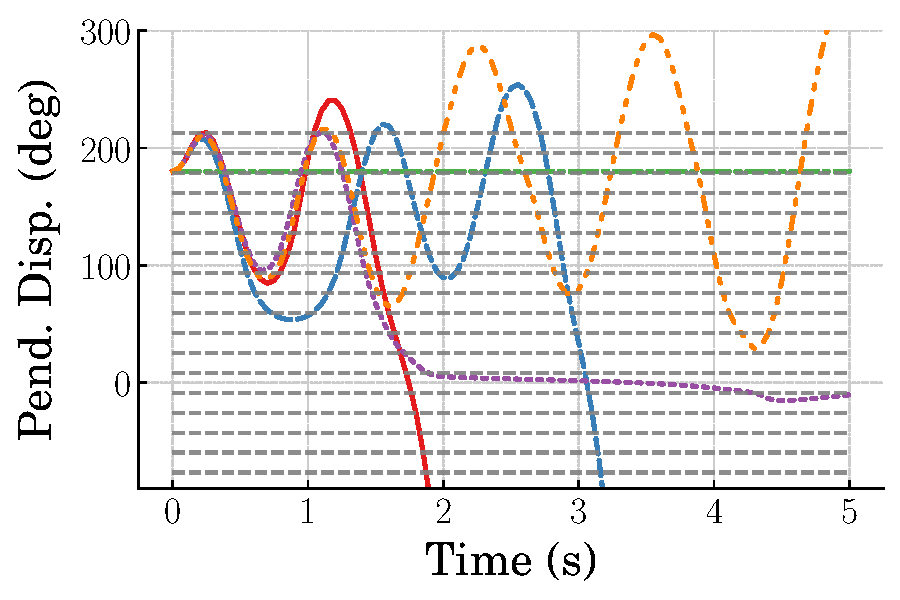
\includegraphics[width=\textwidth]{figures/figures_Interpretability/Mean_ISE_Inverted_Pendulum-v0_cubic_25_bins/Curve_fit_time_responses/pure_RL/curve_fit_Pend_Disp_180.pdf}
        \caption{Curve fit with 25 bins}
        \label{subfig_chap5:inv_pend_pure_RL_180_init_curve_fit_25_bins_unclipped}
    \end{subfigure}
    \hfill
    \caption{Pure RL curve fit responses for $\theta(0)=180^\circ$}
    \label{fig_chap5:inv_pend_pure_RL_180_init_unclipped}
\end{figure}
%

Figure~\ref{fig_chap5:inv_pend_pure_RL_180_init_unclipped} shows time responses for the switching controllers of Pure RL from an initial displacement of $\theta=180^\circ$. Figure~\ref{subfig_chap5:inv_pend_pure_RL_180_init_agent_unclipped} shows the time responses from the neural network controller for reference. The Pure RL switching controller using nine local controllers is shown in Figure~\ref{subfig_chap5:inv_pend_pure_RL_180_init_curve_fit_9_bins_unclipped}. Two of the switching controllers successfully stabilize the system while two other controllers diverge from the equilibrium, contributing to the high ISE. The response shown in blue moves beyond the upper switching boundary for which the local approximations were generated. The switching controller continues using the same local approximation beyond this boundary. Figure~\ref{subfig_chap5:inv_pend_pure_RL_180_init_curve_fit_25_bins_unclipped} shows the performance of the switching controller with nine local controllers. One of the controllers stabilizes the inverted pendulum while the others are unstable.

%
\begin{figure}
    \centering
    \begin{subfigure}[b]{0.32\textwidth}
        \centering
        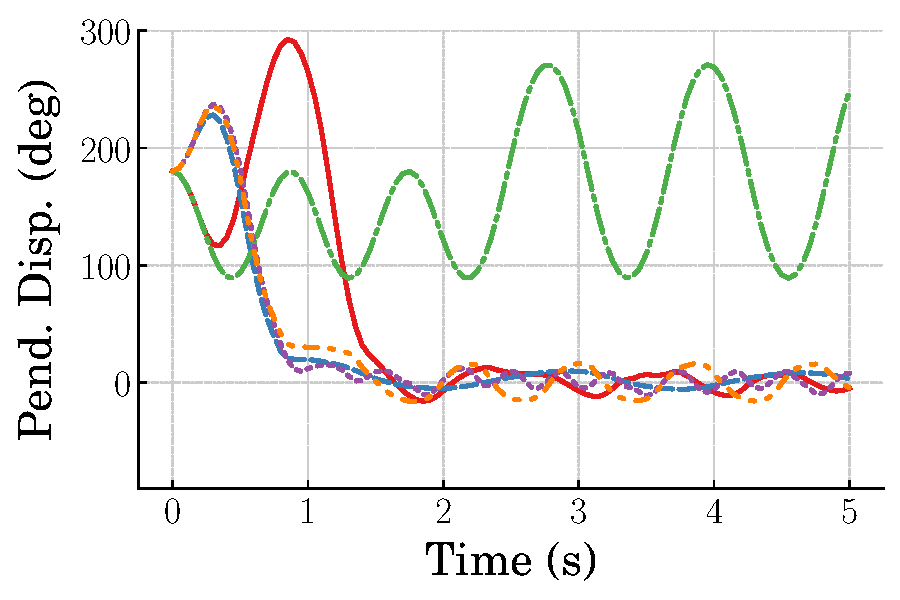
\includegraphics[width=\textwidth]{figures/figures_Interpretability/Mean_ISE_Inverted_Pendulum-v0_cubic_9_bins/Curve_fit_time_responses/lumped_lqr/agent_Pend_Disp_180.pdf}
        \caption{Agent response}
        \label{subfig_chap5:RL_LQR_180_init_agent}
    \end{subfigure}
    \hfill
    \begin{subfigure}[b]{0.32\textwidth}
        \centering
        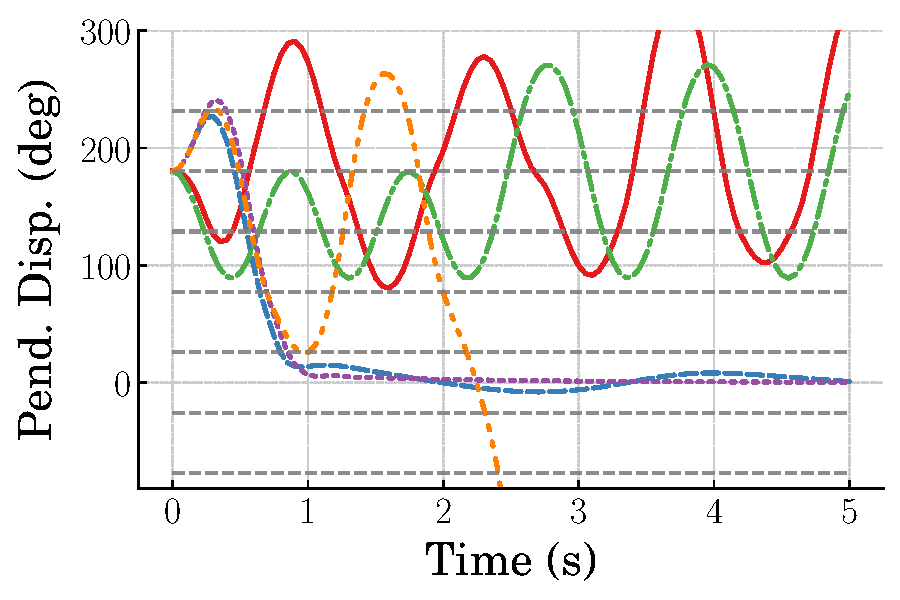
\includegraphics[width=\textwidth]{figures/figures_Interpretability/Mean_ISE_Inverted_Pendulum-v0_cubic_9_bins/Curve_fit_time_responses/lumped_lqr/curve_fit_Pend_Disp_180.pdf}
        \caption{Curve fit with 9 bins}
        \label{subfig_chap5:RL_LQR_180_init_curve_fit_9_bins_unclipped}
    \end{subfigure}
    \hfill
    \begin{subfigure}[b]{0.32\textwidth}
        \centering
        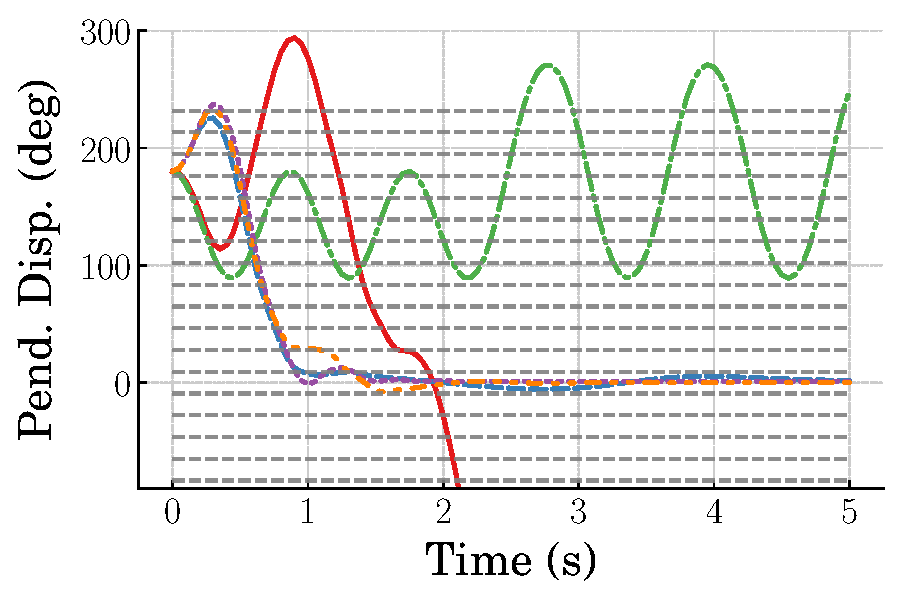
\includegraphics[width=\textwidth]{figures/figures_Interpretability/Mean_ISE_Inverted_Pendulum-v0_cubic_25_bins/Curve_fit_time_responses/lumped_lqr/curve_fit_Pend_Disp_180.pdf}
        \caption{Curve fit with 25 bins}
        \label{subfig_chap5:RL_LQR_180_init_curve_fit_25_bins_unclipped}
    \end{subfigure}
    \hfill
    \caption{RL-LQR curve fit responses for $\theta(0)=180^\circ$}
    \label{fig_chap5:inv_pend_RL_LQR_180_init_unclipped}
\end{figure}
%

Figure~\ref{fig_chap5:inv_pend_RL_LQR_180_init_unclipped} shows the time responses from the switching controllers of RL-LQR from an initial displacement of $\theta=180^\circ$. The controllers with nine local approximations in Figure~\ref{subfig_chap5:RL_LQR_180_init_curve_fit_9_bins_unclipped} have two responses that are stable while the others are unstable. However, none of the responses diverge far from the equilibrium as they do for the nine local controller case for Pure RL. This corresponds to the lower ISE of RL-LQR at $\theta=180^\circ$ in Figure~\ref{subfig_chap5:inv_pend_angle_unclipped_approx_error_9_bins}. The responses for the switching controller with twenty-five local approximations of RL-LQR are shown in Figure~\ref{subfig_chap5:RL_LQR_180_init_curve_fit_25_bins_unclipped}. There are three stabilizing controllers and two unstable responses. Even though there are more stable responses for the RL-LQR case with twenty-five local controllers than for the case with nine local controllers, the ISE for twenty-five local controllers is higher due to one of the responses diverging far from the equilibrium.
%
With the exception of the response that diverges from the equilibrium, the other responses for the switching controller with twenty-five local approximations more closely match the responses from the RL-LQR agent controller compared to the switching controller approximations for Pure RL.
% Although the RL-LQR switching controller approximation has one response that diverges from the equilibrium and another that oscillates near the stable equilibrium (though that one that oscillates about the stable equilibrium is doing what the agent told it to do), these approximations match the RL-LQR agent controllers more closely than the Pure-RL switching controllers.

%
\begin{figure}
    \centering
    \begin{subfigure}[b]{0.32\textwidth}
        \centering
        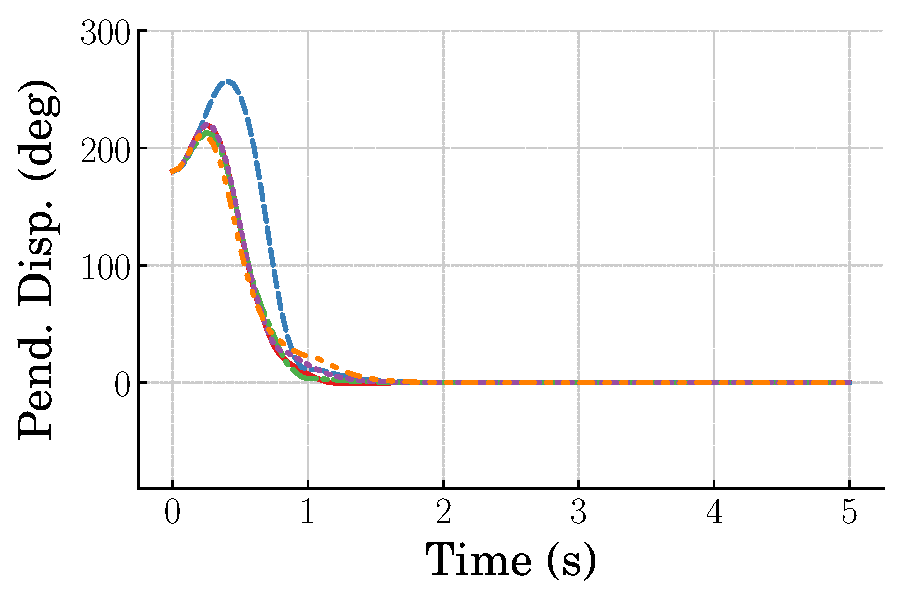
\includegraphics[width=\textwidth]{figures/figures_Interpretability/Mean_ISE_Inverted_Pendulum-v0_cubic_9_bins/Curve_fit_time_responses/switch_lqr/agent_Pend_Disp_180.pdf}
        \caption{Agent response}
        \label{subfig_chap5:S_RL_LQR_180_init_agent}
    \end{subfigure}
    \hfill
    \begin{subfigure}[b]{0.32\textwidth}
        \centering
        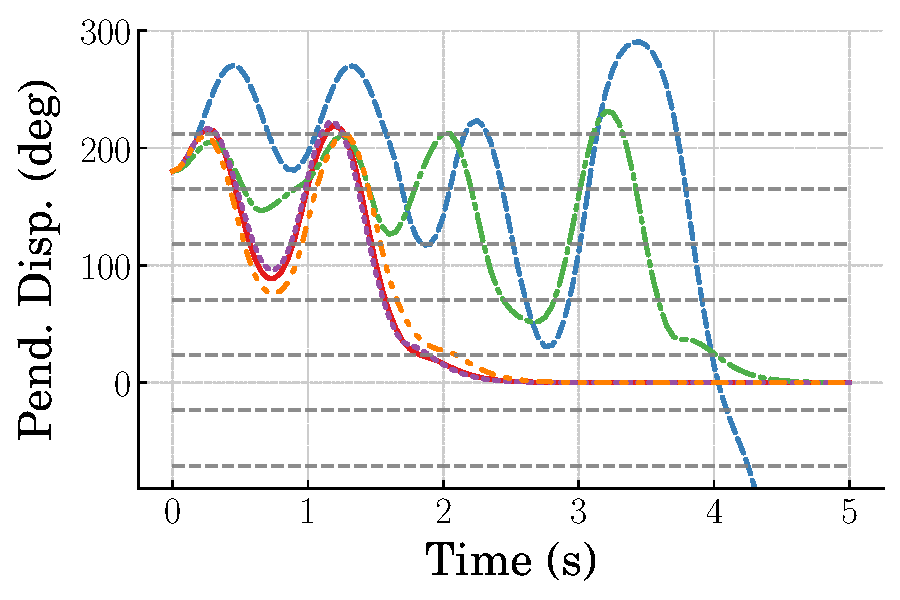
\includegraphics[width=\textwidth]{figures/figures_Interpretability/Mean_ISE_Inverted_Pendulum-v0_cubic_9_bins/Curve_fit_time_responses/switch_lqr/curve_fit_Pend_Disp_180.pdf}
        \caption{Curve fit with 9 bins}
        \label{subfig_chap5:S_RL_LQR_180_init_curve_fit_9_bins_unclipped}
    \end{subfigure}
    \hfill
    \begin{subfigure}[b]{0.32\textwidth}
        \centering
        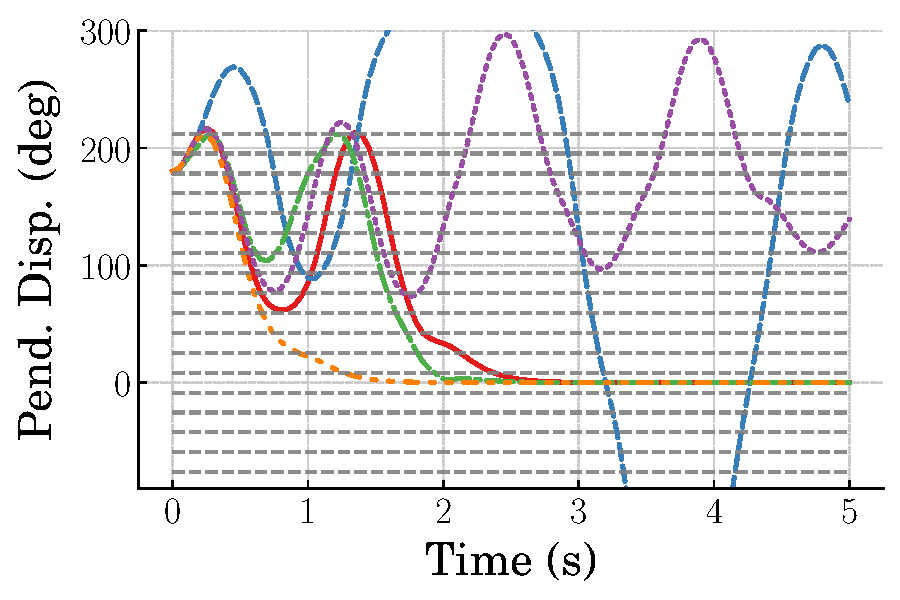
\includegraphics[width=\textwidth]{figures/figures_Interpretability/Mean_ISE_Inverted_Pendulum-v0_cubic_25_bins/Curve_fit_time_responses/switch_lqr/curve_fit_Pend_Disp_180.pdf}
        \caption{Curve fit with 25 bins}
        \label{subfig_chap5:S_RL_LQR_180_init_curve_fit_25_bins_unclipped}
    \end{subfigure}
    \hfill
    \caption{S-RL-LQR curve fit responses for $\theta(0)=180^\circ$}
    \label{fig_chap5:inv_pend_S_RL_LQR_180_init_unclipped}
\end{figure}
%

Figure~\ref{fig_chap5:inv_pend_S_RL_LQR_180_init_unclipped} shows the time responses with the approximations of S-RL-LQR. The approximate controllers use the same switching criteria that was established for switching between the agent action and LQR in the neural network controller.
%
For the switching controller with nine local approximations in Figure~\ref{subfig_chap5:S_RL_LQR_180_init_curve_fit_9_bins_unclipped}, there are four stable responses and one unstable response. Similarly, there are four stable responses for the case with twenty-five local approximations in Figure~\ref{subfig_chap5:S_RL_LQR_180_init_curve_fit_25_bins_unclipped}. Compared to the approximations for Pure RL, the approximations for the S-RL-LQR case were more capable to stabilize the inverted pendulum within the time frame. However, the stabilized responses have higher rise times than the corresponding agent responses.

% %
% \begin{equation}
% \begin{split}
% \hat{u}=(a_{11} + a_{12}x + a_{13}\dot{x} + a_{14}\theta + a_{15}\dot{\theta})x \\ 
% + (a_{21} + a_{22}x + a_{23}\dot{x} + a_{24}\theta + a_{25}\dot{\theta})\dot{x} \\
% + (a_{31} + a_{32}x + a_{33}\dot{x} + a_{34}\theta + a_{35}\dot{\theta})\theta \\
% + (a_{41} + a_{42}x + a_{43}\dot{x} + a_{44}\theta + a_{45}\dot{\theta})\dot{\theta}
% \label{eq_chap5:inv_pend_fit_func}
% \end{split}
% \end{equation}
% %
% This equation allows for linear, polynomial, and \rph{cross multiplication} so there is some variety in the form of the local controllers.
% The RL-LQR approximation seems especially bad, but that seems to be because of high variance in the error. The peak mean ISE of Pure RL seems to tend to be higher than peak mean ISE of S-RL-LQR. \rnotes{Need time responses to explain the high error in some places, and also to provide some intuition into how much error is required for it to be a ``bad'' approximation.} 

% \begin{figure}
%     \centering
%     \begin{subfigure}[b]{0.32\textwidth}
%         \centering
%         \includegraphics[width=\textwidth]{figures/figures_Interpretability/Mean_ISE_Inverted_Pendulum-v0_cubic_9_bins/Curve_fit_time_responses/pure_RL/agent_Pend_Disp_36.pdf}
%         \caption{Agent response}
%         \label{subfig_chap5:inv_pend_angle_approx_error_9_bins}
%     \end{subfigure}
%     \hfill
%     \begin{subfigure}[b]{0.32\textwidth}
%         \centering
%         \includegraphics[width=\textwidth]{figures/figures_Interpretability/Mean_ISE_Inverted_Pendulum-v0_cubic_9_bins/Curve_fit_time_responses/pure_RL/curve_fit_Pend_Disp_36.pdf}
%         \caption{Curve fit with 9 bins}
%         \label{subfig_chap5:inv_pend_angle_approx_error_25_bins}
%     \end{subfigure}
%     \hfill
%     \begin{subfigure}[b]{0.32\textwidth}
%         \centering
%         \includegraphics[width=\textwidth]{figures/figures_Interpretability/Mean_ISE_Inverted_Pendulum-v0_cubic_25_bins/Curve_fit_time_responses/pure_RL/curve_fit_Pend_Disp_36.pdf}
%         \caption{Curve fit with 25 bins}
%         \label{subfig_chap5:inv_pend_angle_approx_error_25_bins}
%     \end{subfigure}
%     \hfill
%     \caption{Example time responses with unsaturated fit function}
%     \label{fig_chap5:inv_pend_unclipped_approx_error}
% \end{figure}

In summary, the performance of the switching controllers for RL-LQR most closely matched the corresponding agent controllers from $\theta(0)=180^\circ$ despite the high ISE. The switching controller approximations for S-RL-LQR were less accurate than RL-LQR, but were more accurate than Pure RL. While a few of the responses with the switching controllers were adequately accurate to match the agent responses, many were not adequately accurate. This inconsistency caused the high standard deviation and spikes in the mean ISE seen in Figure~\ref{fig_chap5:inv_pend_angle_unclipped_approx_error}. Additionally, some switching controllers that were stabilizing for one set of local approximations were not stabilizing for corresponding switching controllers with a different number of local approximations. The inconsistency of fit accuracy among different initial conditions and different sizes of the switching controllers indicates the fit is very sensitive to these factors. There may also be better candidates for local approximation functions to use for curve fits.

\subsubsection{Approximation Near the Equilibrium}

The widest regions for which Mean ISE is low for the inverted pendulum switching controllers are for initial conditions near the equilibrium, $\theta=0$. It is therefore beneficial to split the analysis of the curve fits into categories of near equilibrium and not near equilibrium.
%
Figure~\ref{fig_chap5:Mean_ISE_near_equil} shows the mean ISE for $-45^\circ\le\theta\le45^\circ$.
% Another state-action data was populated from responses with initial angular displacements between $-45^\circ\le\theta \le45^\circ$}.
%
There is no error between the approximations and the agent controllers for S-RL-LQR since this is the region for which the S-RL-LQR controller uses only LQR.
% This corresponds to the region for which S-RL-LQR uses LQR, so there is no error between the responses from the agent and the curve fits.
Figure~\ref{subfig_chap5:near_equil_1_bins_unclipped} shows the ISE when only one approximated controller is used for each agent. The Pure RL approximations have low error for most of the range except near the extremes. The case with only one approximate control law for the entire range has the widest region of low mean ISE, with the increase in the number of approximations used reducing the range for which the ISE is low. As was common with the other approximations, the switching controllers for RL-LQR have high mean error and variance in this region and do not show a clear trend in performance of the approximations.
%
However, in contrast to the Pure RL approximations, the mean ISE for the RL-LQR approximations is lowest for the case with five local approximations and is higher for decreases in the number of local controller approximations.

%
\begin{figure}
    \centering
    \begin{subfigure}[b]{0.32\textwidth}
        \centering
        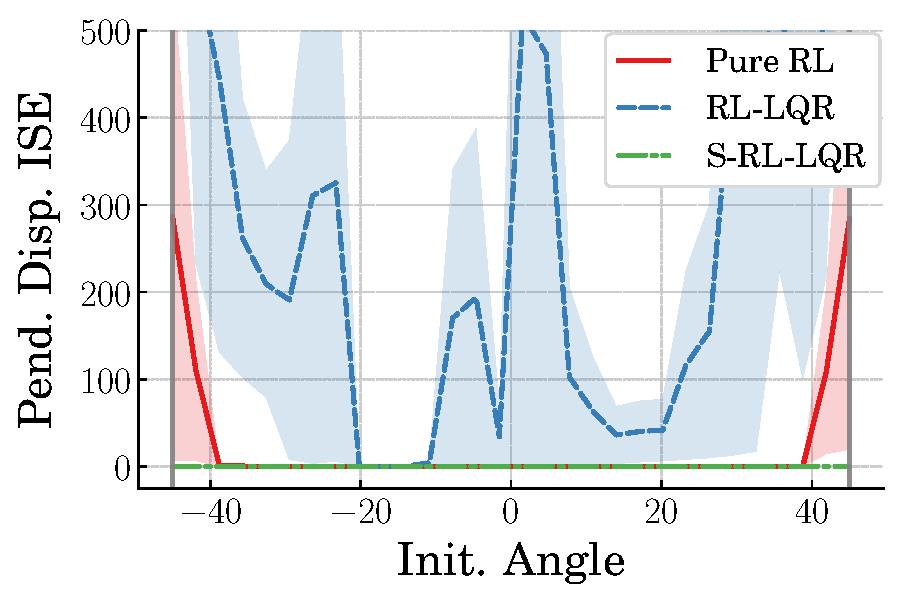
\includegraphics[width=\textwidth]{figures/figures_Interpretability/Mean_ISE_Inverted_Pendulum-v0_cubic_1_bins_near_equil/Mean_ISE_Inverted_Pendulum-v0_cubic_Pend_Disp_1_bins.pdf}
        \caption{1 approximation}
        \label{subfig_chap5:near_equil_1_bins_unclipped}
    \end{subfigure}
    \hfill
    \begin{subfigure}[b]{0.32\textwidth}
        \centering
        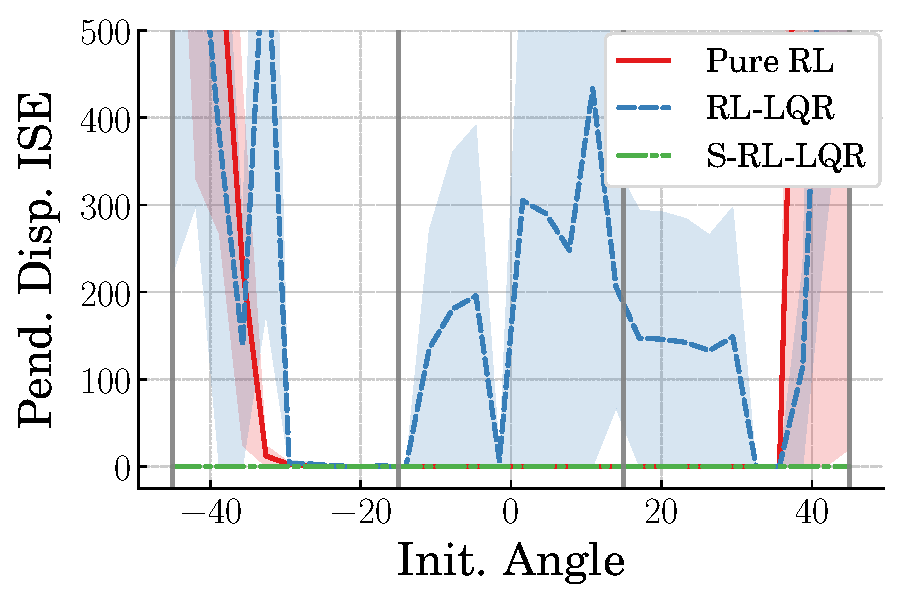
\includegraphics[width=\textwidth]{figures/figures_Interpretability/Mean_ISE_Inverted_Pendulum-v0_cubic_3_bins_near_equil/Mean_ISE_Inverted_Pendulum-v0_cubic_Pend_Disp_3_bins.pdf}
        \caption{3 approximations}
        \label{subfig_chap5:near_equil_3_bins_unclipped}
    \end{subfigure}
    \hfill
    \begin{subfigure}[b]{0.32\textwidth}
        \centering
        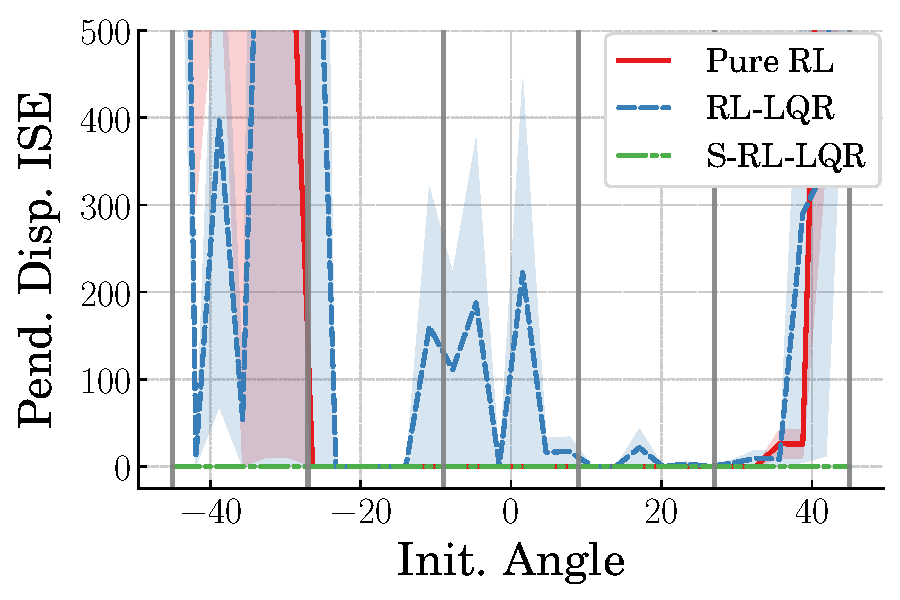
\includegraphics[width=\textwidth]{figures/figures_Interpretability/Mean_ISE_Inverted_Pendulum-v0_cubic_5_bins_near_equil/Mean_ISE_Inverted_Pendulum-v0_cubic_Pend_Disp_5_bins.pdf}
        \caption{5 approximations}
        \label{subfig_chap5:near_equil_5_bins_unclipped}
    \end{subfigure}
    \caption{ISE of inverted pendulum local controllers for $\theta(0)=45^\circ$}
    \label{fig_chap5:Mean_ISE_near_equil}
\end{figure}
%

%
\begin{figure}
    \centering
    \begin{subfigure}[b]{0.32\textwidth}
        \centering
        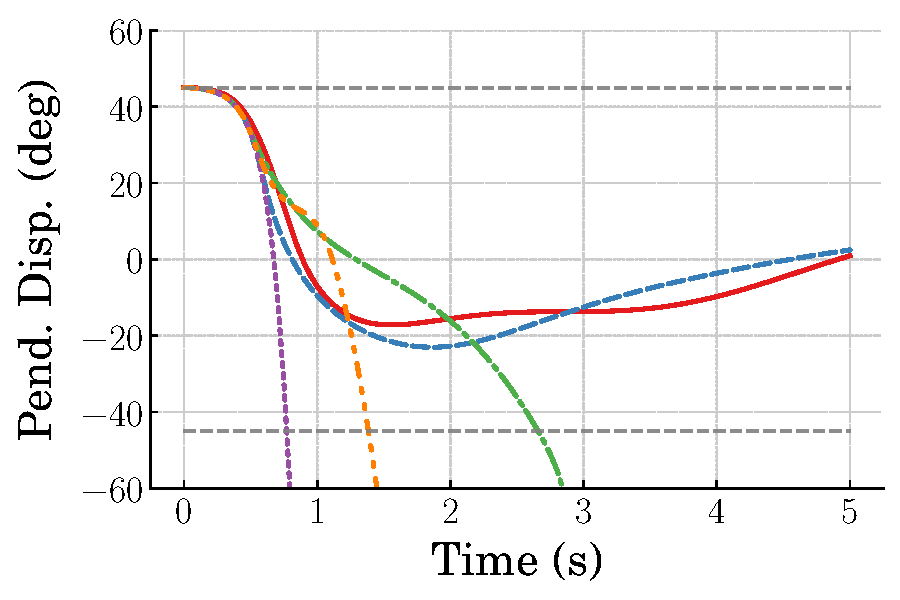
\includegraphics[width=\textwidth]{figures/figures_Interpretability/Mean_ISE_Inverted_Pendulum-v0_cubic_1_bins_near_equil/Curve_fit_time_responses/pure_RL/curve_fit_Pend_Disp_45.pdf}
        \caption{1 approximation}
        \label{subfig_chap5:pure_RL_near_equil_1_bins_resp_unclipped}
    \end{subfigure}
    \hfill
    \begin{subfigure}[b]{0.32\textwidth}
        \centering
        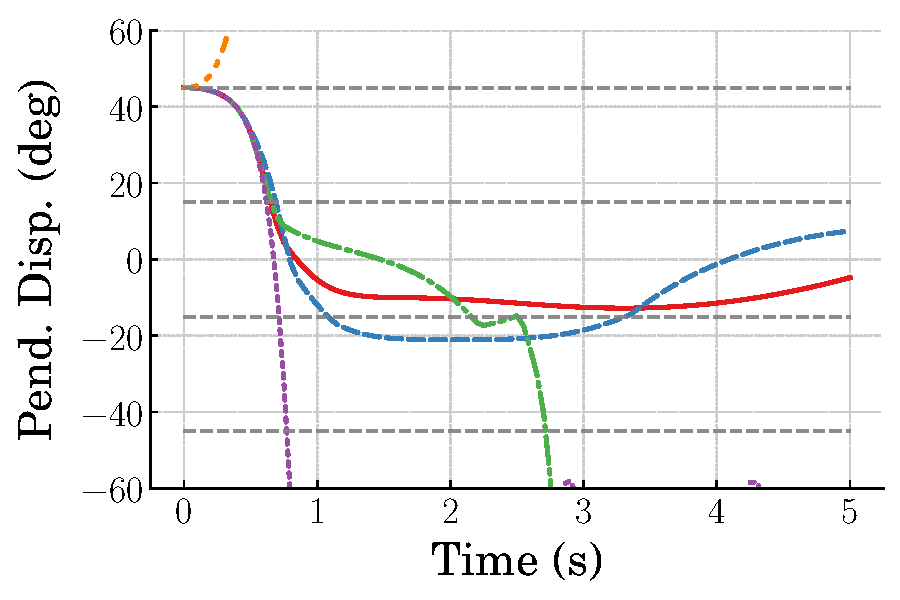
\includegraphics[width=\textwidth]{figures/figures_Interpretability/Mean_ISE_Inverted_Pendulum-v0_cubic_3_bins_near_equil/Curve_fit_time_responses/pure_RL/curve_fit_Pend_Disp_45.pdf}
        \caption{3 approximations}
        \label{subfig_chap5:pure_RL_near_equil_3_bins_resp_unclipped}
    \end{subfigure}
    \hfill
    \begin{subfigure}[b]{0.32\textwidth}
        \centering
        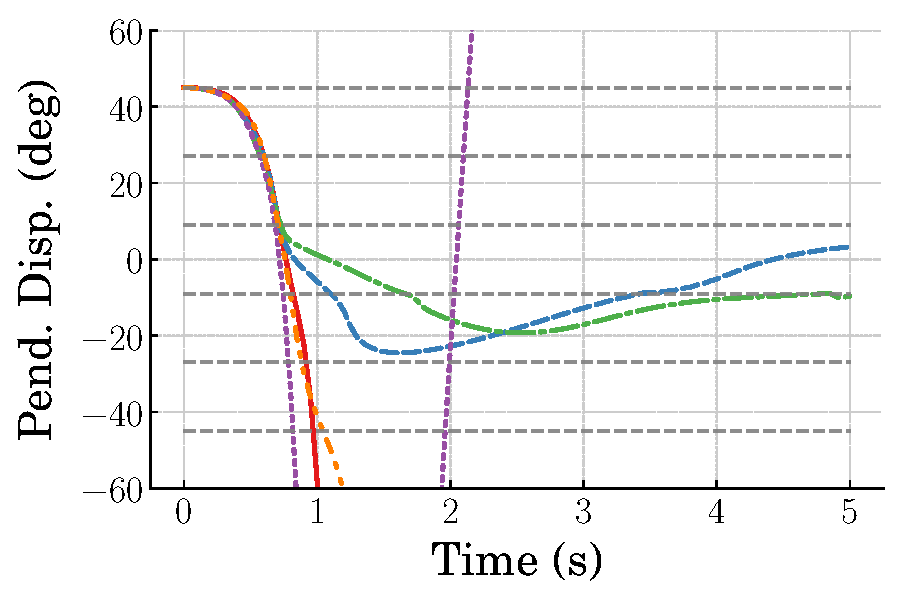
\includegraphics[width=\textwidth]{figures/figures_Interpretability/Mean_ISE_Inverted_Pendulum-v0_cubic_5_bins_near_equil/Curve_fit_time_responses/pure_RL/curve_fit_Pend_Disp_45.pdf}
        \caption{5 approximations}
        \label{subfig_chap5:pure_RL_near_equil_5_bins_resp_unclipped}
    \end{subfigure}
    \caption{Switching controller responses for Pure RL for $\theta(0)=45^\circ$}
    \label{fig_chap5:pure_RL_near_equil_45_resp_unclipped}
\end{figure}
%
Time responses of the switching controllers for Pure RL are shown in Figure~\ref{fig_chap5:pure_RL_near_equil_45_resp_unclipped}. These responses start from rest with initial angular displacement of $\theta=45^\circ$.
For the case with only one local approximation in Figure~\ref{subfig_chap5:pure_RL_near_equil_1_bins_resp_unclipped},
only two responses remain near the equilibrium.
%
For the switching controller with three local approximations in Figure~\ref{subfig_chap5:pure_RL_near_equil_3_bins_resp_unclipped}, only two responses remain near the equilibrium, similar to the case with one local approximation.
%
For the case with five local approximations in Figure~\ref{subfig_chap5:pure_RL_near_equil_5_bins_resp_unclipped}, two of the responses remain near the equilibrium.
However, the response in red that previously remained near the equilibrium for the other cases diverges for this case.
This shows that the conditions necessary to generate good approximations are not identical for the different agents.
% In terms of how many responses diverge from the equilibrium, there is little difference between the responses based on the number of piecewise approximations. For all three switching controllers, three of the responses diverge away from the equilibrium, contributing to the high mean ISE and standard deviation in Figure~\ref{fig_chap5:Mean_ISE_near_equil}. While the responses indicated by the red (solid) and blue (dashed) lines remain near the equilibrium in Figure~\ref{subfig_chap5:pure_RL_near_equil_1_bins_resp_unclipped} and Figure~\ref{subfig_chap5:pure_RL_near_equil_3_bins_resp_unclipped}, the response indicated in red diverges in Figure~\ref{subfig_chap5:pure_RL_near_equil_5_bins_resp_unclipped} while the response shown by the green (dash-dot) line remains near the equilibrium. \rph{The divergence from the equilibrium and the inconsistency of the responses indicate that a cubic polynomial is not a good candidate function for the agents in the area near $\theta=45^\circ$. \rnotes{It may also be that we need more data.}}
%
Figure~\ref{fig_chap5:lumped_LQR_near_equil_45_resp_unclipped} shows the time responses with initial displacements of $\theta(0)=45^\circ$ for the switching controller approximation for RL-LQR. For all cases shown, none of the approximated controllers are stabilizing.
% \rph{The responses are similar to the those of the Pure RL approximations. The responses for one local approximation in Figure~\ref{subfig_chap5:lumped_LQR_near_equil_1_bins_resp_unclipped} have no responses that settle near the equilibrium. Figure~\ref{subfig_chap5:lumped_LQR_near_equil_3_bins_resp_unclipped} for three local controllers has one that settles at the equilibrium. Figure~\ref{subfig_chap5:lumped_LQR_near_equil_5_bins_resp_unclipped} for five local controllers has no responses that settle near the equilibrium.}
%
\begin{figure}
    \centering
    \begin{subfigure}[b]{0.32\textwidth}
        \centering
        \includegraphics[width=\textwidth]{figures/figures_Interpretability/Mean_ISE_Inverted_Pendulum-v0_cubic_1_bins_near_equil/Curve_fit_time_responses/lumped_LQR/curve_fit_Pend_Disp_45.pdf}
        \caption{1 approximation}
        \label{subfig_chap5:lumped_LQR_near_equil_1_bins_resp_unclipped}
    \end{subfigure}
    \hfill
    \begin{subfigure}[b]{0.32\textwidth}
        \centering
        \includegraphics[width=\textwidth]{figures/figures_Interpretability/Mean_ISE_Inverted_Pendulum-v0_cubic_3_bins_near_equil/Curve_fit_time_responses/lumped_LQR/curve_fit_Pend_Disp_45.pdf}
        \caption{3 approximations}
        \label{subfig_chap5:lumped_LQR_near_equil_3_bins_resp_unclipped}
    \end{subfigure}
    \hfill
    \begin{subfigure}[b]{0.32\textwidth}
        \centering
        \includegraphics[width=\textwidth]{figures/figures_Interpretability/Mean_ISE_Inverted_Pendulum-v0_cubic_5_bins_near_equil/Curve_fit_time_responses/lumped_LQR/curve_fit_Pend_Disp_45.pdf}
        \caption{5 approximations}
        \label{subfig_chap5:lumped_LQR_near_equil_5_bins_resp_unclipped}
    \end{subfigure}
    \caption{Switching controller response for RL-LQR for $\theta(0)=45^\circ$}
    \label{fig_chap5:lumped_LQR_near_equil_45_resp_unclipped}
\end{figure}
%

Based on the plots for mean ISE near equilibrium, the response error tends to be lower for initial angular displacements closer to $\theta=0$.
Figure~\ref{fig_chap5:pure_RL_near_equil_15_resp_unclipped} shows the time responses from Pure RL curve fits for an initial condition of $\theta=15^\circ$. All responses from this initial condition stay near the equilibrium as was expected from the Mean ISE in Figure~\ref{fig_chap5:Mean_ISE_near_equil}, and there is more consistency in the behaviors of the approximations with different numbers of local controllers.
%
\begin{figure}[tb]
    \centering
    \begin{subfigure}[b]{0.32\textwidth}
        \centering
        \includegraphics[width=\textwidth]{figures/figures_Interpretability/Mean_ISE_Inverted_Pendulum-v0_cubic_1_bins_near_equil/Curve_fit_time_responses/pure_RL/curve_fit_Pend_Disp_15.pdf}
        \caption{1 approximation}
        \label{subfig_chap5:pure_RL_near_equil_15_1_bins_resp_unclipped}
    \end{subfigure}
    \hfill
    \begin{subfigure}[b]{0.32\textwidth}
        \centering
        \includegraphics[width=\textwidth]{figures/figures_Interpretability/Mean_ISE_Inverted_Pendulum-v0_cubic_3_bins_near_equil/Curve_fit_time_responses/pure_RL/curve_fit_Pend_Disp_15.pdf}
        \caption{3 approximations}
        \label{subfig_chap5:pure_RL_near_equil_15_3_bins_resp_unclipped}
    \end{subfigure}
    \hfill
    \begin{subfigure}[b]{0.32\textwidth}
        \centering
        \includegraphics[width=\textwidth]{figures/figures_Interpretability/Mean_ISE_Inverted_Pendulum-v0_cubic_5_bins_near_equil/Curve_fit_time_responses/pure_RL/curve_fit_Pend_Disp_15.pdf}
        \caption{5 approximations}
        \label{subfig_chap5:pure_RL_near_equil_15_5_bins_resp_unclipped}
    \end{subfigure}
    \caption{Switching controller response for Pure RL for $\theta(0)=15^\circ$}
    \label{fig_chap5:pure_RL_near_equil_15_resp_unclipped}
\end{figure}
%

The responses of the switching controllers for RL-LQR from an initial angular displacement of $\theta=15^\circ$ are shown in Figure~\ref{fig_chap5:lumped_LQR_near_equil_15_resp_unclipped}. Two of the responses diverge from the equilibrium in Figure~\ref{subfig_chap5:lumped_LQR_near_equil_15_1_bins_resp_unclipped}. However, two settle at the equilibrium and another oscillates about the equilibrium. In Figure~\ref{subfig_chap5:lumped_LQR_near_equil_15_3_bins_resp_unclipped}, three of the responses remain near the equilibrium in the time range shown. However, two of the responses are unstable and the response in blue begins to diverge away from the equilibrium. In Figure~\ref{subfig_chap5:lumped_LQR_near_equil_15_5_bins_resp_unclipped}, only four of the five responses remain near the equilibrium during the time range shown.
%
\begin{figure}[tb]
    \centering
    \begin{subfigure}[b]{0.32\textwidth}
        \centering
        \includegraphics[width=\textwidth]{figures/figures_Interpretability/Mean_ISE_Inverted_Pendulum-v0_cubic_1_bins_near_equil/Curve_fit_time_responses/lumped_LQR/curve_fit_Pend_Disp_15.pdf}
        \caption{1 approximation}
        \label{subfig_chap5:lumped_LQR_near_equil_15_1_bins_resp_unclipped}
    \end{subfigure}
    \hfill
    \begin{subfigure}[b]{0.32\textwidth}
        \centering
        \includegraphics[width=\textwidth]{figures/figures_Interpretability/Mean_ISE_Inverted_Pendulum-v0_cubic_3_bins_near_equil/Curve_fit_time_responses/lumped_LQR/curve_fit_Pend_Disp_15.pdf}
        \caption{3 approximations}
        \label{subfig_chap5:lumped_LQR_near_equil_15_3_bins_resp_unclipped}
    \end{subfigure}
    \hfill
    \begin{subfigure}[b]{0.32\textwidth}
        \centering
        \includegraphics[width=\textwidth]{figures/figures_Interpretability/Mean_ISE_Inverted_Pendulum-v0_cubic_5_bins_near_equil/Curve_fit_time_responses/lumped_LQR/curve_fit_Pend_Disp_15.pdf}
        \caption{5 approximations}
        \label{subfig_chap5:lumped_LQR_near_equil_15_5_bins_resp_unclipped}
    \end{subfigure}
    \caption{Switching controller response for RL-LQR for $\theta(0)=15^\circ$}
    \label{fig_chap5:lumped_LQR_near_equil_15_resp_unclipped}
\end{figure}
%

Although the approximate controllers for the crane were generally able to provide accurate responses that closely matched the behavior of the agents, the approximate controllers for the inverted pendulum tended to have less accuracy. In addition to this, behavior was often inconsistent, where approximations were stable for one switching controller and unstable for another switching controller with a different number of local approximations.
This suggests that the polynomial fit function was a poor choice to approximate the agents for the inverted pendulum controllers.
% This shows a need to manually tune the parameters to generate approximations for each agent.

% \rnotes{Most likely comment out everything below.}

% It is desirable to have a general fit function that works consistently for a range of settings. This motivates trying different fit functions to determine what is better. The \rph{set/replay buffer} used to generate the curve fits for the switching controllers is subject to saturation. For the previous time responses, it was ensured that the switching controllers did not exceed the prescribed actuator limits. However, the fit function itself was continuous with no output constraints. A better curve fit may be achieved by using a fit function that \rph{exhibits saturation}.

% \begin{equation}
% \hat{a}_l=\textbf{sat}\left(\sum_{i=0}^p a_ix^i + b_i\dot{x}^i + c_i\theta^i + d_i\dot{\theta}^i \right)
% \label{eq_chap5:inv_pend_sat_approx_func}
% \end{equation}

% \begin{figure}
%      \centering
%      \begin{subfigure}[b]{0.49\textwidth}
%          \centering
%          \includegraphics[width=\textwidth]{figures/figures_Interpretability/Mean_ISE_Inverted_Pendulum-v0_clipped_cubic_9_bins/Mean_ISE_Inverted_Pendulum-v0_clipped_cubic_Pend_Disp_9_bins.pdf}
%          \caption{9 local approximations}
%          \label{subfig_chap5:inv_pend_angle_clipped_approx_error_9_bins}
%      \end{subfigure}
%      \hfill
%      \begin{subfigure}[b]{0.49\textwidth}
%          \centering
%          \includegraphics[width=\textwidth]{figures/figures_Interpretability/Mean_ISE_Inverted_Pendulum-v0_clipped_cubic_25_bins/Mean_ISE_Inverted_Pendulum-v0_clipped_cubic_Pend_Disp_25_bins}
%          \caption{25 local approximations}
%          \label{subfig_chap5:inv_pend_angle_clipped_approx_error_25_bins}
%      \end{subfigure}
%         \caption{Time response error with saturated 3 degree polynomial local controllers}
%         \label{fig_chap5:inv_pend_angle_clipped_approx_error}
% \end{figure}
% %

% %
% \begin{figure}
%     \centering
%     \begin{subfigure}[b]{0.32\textwidth}
%         \centering
%         \includegraphics[width=\textwidth]{figures/figures_Interpretability/Mean_ISE_Inverted_Pendulum-v0_clipped_cubic_9_bins/Curve_fit_time_responses/pure_RL/agent_Pend_Disp_180.pdf}
%         \caption{Agent response}
%         \label{subfig_chap5:inv_pend_pure_RL_180_init_agent}
%     \end{subfigure}
%     \hfill
%     \begin{subfigure}[b]{0.32\textwidth}
%         \centering
%         \includegraphics[width=\textwidth]{figures/figures_Interpretability/Mean_ISE_Inverted_Pendulum-v0_clipped_cubic_9_bins/Curve_fit_time_responses/pure_RL/curve_fit_Pend_Disp_180.pdf}
%         \caption{Curve fit with 9 bins}
%         \label{subfig_chap5:inv_pend_pure_RL_180_init_curve_fit_9_bins_clipped}
%     \end{subfigure}
%     \hfill
%     \begin{subfigure}[b]{0.32\textwidth}
%         \centering
%         \includegraphics[width=\textwidth]{figures/figures_Interpretability/Mean_ISE_Inverted_Pendulum-v0_clipped_cubic_25_bins/Curve_fit_time_responses/pure_RL/curve_fit_Pend_Disp_180.pdf}
%         \caption{Curve fit with 25 bins}
%         \label{subfig_chap5:inv_pend_pure_RL_180_init_curve_fit_25_bins_clipped}
%     \end{subfigure}
%     \hfill
%     \caption{Pure RL saturated curve fit time responses from $\theta=180^\circ$}
%     \label{fig_chap5:inv_pend_pure_RL_180_init_clipped}
% \end{figure}
% %

% %
% \begin{figure}
%     \centering
%     \begin{subfigure}[b]{0.32\textwidth}
%         \centering
%         \includegraphics[width=\textwidth]{figures/figures_Interpretability/Mean_ISE_Inverted_Pendulum-v0_clipped_cubic_9_bins/Curve_fit_time_responses/lumped_lqr/agent_Pend_Disp_180.pdf}
%         \caption{Agent response}
%         \label{subfig_chap5:RL_LQR_180_init_agent}
%     \end{subfigure}
%     \hfill
%     \begin{subfigure}[b]{0.32\textwidth}
%         \centering
%         \includegraphics[width=\textwidth]{figures/figures_Interpretability/Mean_ISE_Inverted_Pendulum-v0_clipped_cubic_9_bins/Curve_fit_time_responses/lumped_lqr/curve_fit_Pend_Disp_180.pdf}
%         \caption{Curve fit with 9 bins}
%         \label{subfig_chap5:RL_LQR_180_init_curve_fit_9_bins_clipped}
%     \end{subfigure}
%     \hfill
%     \begin{subfigure}[b]{0.32\textwidth}
%         \centering
%         \includegraphics[width=\textwidth]{figures/figures_Interpretability/Mean_ISE_Inverted_Pendulum-v0_clipped_cubic_25_bins/Curve_fit_time_responses/lumped_lqr/curve_fit_Pend_Disp_180.pdf}
%         \caption{Curve fit with 25 bins}
%         \label{subfig_chap5:RL_LQR_180_init_curve_fit_25_bins_clipped}
%     \end{subfigure}
%     \hfill
%     \caption{RL-LQR saturated curve fit time responses from $\theta=180^\circ$}
%     \label{fig_chap5:inv_pend_RL_LQR_180_init_clipped}
% \end{figure}
% %

% %
% \begin{figure}
%     \centering
%     \begin{subfigure}[b]{0.32\textwidth}
%         \centering
%         \includegraphics[width=\textwidth]{figures/figures_Interpretability/Mean_ISE_Inverted_Pendulum-v0_clipped_cubic_9_bins/Curve_fit_time_responses/switch_lqr/agent_Pend_Disp_180.pdf}
%         \caption{Agent response}
%         \label{subfig_chap5:S_RL_LQR_180_init_agent}
%     \end{subfigure}
%     \hfill
%     \begin{subfigure}[b]{0.32\textwidth}
%         \centering
%         \includegraphics[width=\textwidth]{figures/figures_Interpretability/Mean_ISE_Inverted_Pendulum-v0_clipped_cubic_9_bins/Curve_fit_time_responses/switch_lqr/curve_fit_Pend_Disp_180.pdf}
%         \caption{Curve fit with 9 bins}
%         \label{subfig_chap5:S_RL_LQR_180_init_curve_fit_9_bins_clipped}
%     \end{subfigure}
%     \hfill
%     \begin{subfigure}[b]{0.32\textwidth}
%         \centering
%         \includegraphics[width=\textwidth]{figures/figures_Interpretability/Mean_ISE_Inverted_Pendulum-v0_clipped_cubic_25_bins/Curve_fit_time_responses/switch_lqr/curve_fit_Pend_Disp_180.pdf}
%         \caption{Curve fit with 25 bins}
%         \label{subfig_chap5:S_RL_LQR_180_init_curve_fit_25_bins_clipped}
%     \end{subfigure}
%     \hfill
%     \caption{S-RL-LQR saturated curve fit time responses from $\theta=180^\circ$}
%     \label{fig_chap5:inv_pend_S_RL_LQR_180_init_clipped}
% \end{figure}
% %

% % %
% % \begin{figure}
% %     \centering
% %     \begin{subfigure}[b]{0.49\textwidth}
% %         \centering
% %         \includegraphics[width=\textwidth]{figures/figures_Interpretability/Mean_ISE_Inverted_Pendulum-v0_cubic_3_bins_near_equil/Mean_ISE_Inverted_Pendulum-v0_cubic_Pend_Disp_3_bins.pdf}
% %         \caption{3 approximations}
% %         \label{subfig_chap5:near_equil_3_bins_unclipped}
% %     \end{subfigure}
% %     \hfill
% %     \begin{subfigure}[b]{0.49\textwidth}
% %         \centering
% %         \includegraphics[width=\textwidth]{figures/figures_Interpretability/Mean_ISE_Inverted_Pendulum-v0_cubic_5_bins_near_equil/Mean_ISE_Inverted_Pendulum-v0_cubic_Pend_Disp_5_bins.pdf}
% %         \caption{5 approximations}
% %         \label{subfig_chap5:near_equil_5_bins_unclipped}
% %     \end{subfigure}
% %     \hfill
% %     \begin{subfigure}[b]{0.49\textwidth}
% %         \centering
% %         \includegraphics[width=\textwidth]{figures/figures_Interpretability/Mean_ISE_Inverted_Pendulum-v0_clipped_cubic_3_bins_near_equil/Mean_ISE_Inverted_Pendulum-v0_clipped_cubic_Pend_Disp_3_bins.pdf}
% %         \caption{3 approximations with saturated function}
% %         \label{subfig_chap5:near_equil_3_bins_clipped}
% %     \end{subfigure}
% %     \hfill
% %     \begin{subfigure}[b]{0.49\textwidth}
% %         \centering
% %         \includegraphics[width=\textwidth]{figures/figures_Interpretability/Mean_ISE_Inverted_Pendulum-v0_clipped_cubic_5_bins_near_equil/Mean_ISE_Inverted_Pendulum-v0_clipped_cubic_Pend_Disp_5_bins.pdf}
% %         \caption{5 approximations with saturated function}
% %         \label{subfig_chap5:near_equil_5_bins_clipped}
% %     \end{subfigure}
% %     \caption{Mean ISE near equilibrium}
% %     \label{fig_chap5:Mean_ISE_near_equil}
% % \end{figure}
% % %

% \rnotes{Include Mean ISE for 1 bin case, remove clipped results. Explain how the response error is being caused by switching conditions. That is why 1 bin works decently well for Pure RL. Add some time responses from $45^\circ$ and $30^\circ$. From there we discuss the need for a better fit function that handles the nonlinearity more accurately. If I can get sliding mode control to work, I may be able to show those results. I should be able to apply the same thing for the other controllers for the other systems.}

% % \begin{figure}
% %     \centering
% %     \begin{subfigure}[b]{0.32\textwidth}
% %         \centering
% %         \includegraphics[width=\textwidth]{figures/figures_Interpretability/Mean_ISE_Inverted_Pendulum-v0_clipped_cubic_9_bins/Curve_fit_time_responses/pure_RL/agent_Pend_Disp_36.pdf}
% %         \caption{Agent response}
% %         \label{subfig_chap5:inv_pend_angle_approx_error_9_bins}
% %     \end{subfigure}
% %     \hfill
% %     \begin{subfigure}[b]{0.32\textwidth}
% %         \centering
% %         \includegraphics[width=\textwidth]{figures/figures_Interpretability/Mean_ISE_Inverted_Pendulum-v0_clipped_cubic_9_bins/Curve_fit_time_responses/pure_RL/curve_fit_Pend_Disp_36.pdf}
% %         \caption{Curve fit with 9 bins}
% %         \label{subfig_chap5:inv_pend_angle_approx_error_25_bins}
% %     \end{subfigure}
% %     \hfill
% %     \begin{subfigure}[b]{0.32\textwidth}
% %         \centering
% %         \includegraphics[width=\textwidth]{figures/figures_Interpretability/Mean_ISE_Inverted_Pendulum-v0_clipped_cubic_25_bins/Curve_fit_time_responses/pure_RL/curve_fit_Pend_Disp_36.pdf}
% %         \caption{Curve fit with 25 bins}
% %         \label{subfig_chap5:inv_pend_angle_approx_error_25_bins}
% %     \end{subfigure}
% %     \hfill
% %     \caption{Example time responses with saturated fit function}
% %     \label{fig_chap5:inv_pend_unclipped_approx_error}
% % \end{figure}

% \rnotes{Are the agents of certain control structures easier to approximate with the gain scheduled approximation? Are they more accurate?}

% \rnotes{Can I use this setup for some kind of stability analysis?}

% \rnotes{Can I modify the gain scheduled approximation to produce an asymptotically stable approximation?}

% \rnotes{Should I produce a ``replay buffer'' for the switching controller approximation and compare to the buffer for agent?}

\section{Agent Output Contributions}
%
\begin{figure}[tb]
    \centering
    \begin{subfigure}[b]{0.49\textwidth}
        \centering
        \includegraphics[width=\textwidth]{figures/figures_Interpretability/Invpend_contours/agent_contours_Trolly_Disp_trial_0.pdf}
        \caption{Cart Displacement}
        \label{subfig_chap5:agent_contribution_contours_trolley_disp}
    \end{subfigure}
    \hfill
    \begin{subfigure}[b]{0.49\textwidth}
        \centering
        \includegraphics[width=\textwidth]{figures/figures_Interpretability/Invpend_contours/agent_contours_Trolley_Vel_trial_0}
        \caption{Cart Velocity}
        \label{subfig_chap5:agent_contribution_contours_trolley_vel}
    \end{subfigure}
    \hfill
    \begin{subfigure}[b]{0.49\textwidth}
        \centering
        \includegraphics[width=\textwidth]{figures/figures_Interpretability/Invpend_contours/agent_contours_Pend_Vel_trial_0.pdf}
        \caption{Pendulum Velocity}
        \label{subfig_chap5:agent_contribution_contours_pend_vel}
    \end{subfigure}
    \caption{Inverted pendulum agent contributions for different states}
    \label{fig_chap5:agent_contribution_contours}
\end{figure}
%
The switching controllers in this chapter were all generated by modeling the contributions from all states using the same fit function. Using a generalized fit function to approximate the contribution from the switching variable is appropriate since only a small range of the variable is used for each local approximation. However, there is an indefinite range for the other states within each subset of the operating space. Generic fit functions may not always be appropriate for potentially wide ranges of states, especially as the controller switches between different local approximations.
%
The unsuitability of generic fit functions can be illustrated in Figure~\ref{fig_chap5:agent_contribution_contours}, which plots state contributions to the output of an agent for the inverted pendulum.
% The results above were acquired by using the same fit function to approximate the contribution of all states to the agent output. Using a generalized fit function to approximate the contribution from the switching variable is appropriate since only a small range of the variable is used for each local approximation. However, within each subset of the operating space, there is an indefinite range for the other states.
% Generic fit functions may not always be appropriate for these wider ranges, especially as the controller switches between different local approximations.
% This is illustrated in Figure~\ref{fig_chap5:agent_contribution_contours}, which plots the state contribution to the output of an agent for the inverted pendulum.
The range of the state in question is shown on the horizontal axis. Each line shows the agent output for a fixed value of the switching variable with all other states equal to zero. Although a third-order polynomial was used to approximate all state contributions, this generic function would be unable to accurately approximate all of the agent outputs. This suggests that some initial interpretation of the behavior of the agent is necessary in order to manually generate appropriate curvefit functions for the agents.
% \begin{itemize}
%     \item The results above were acquired from using the same functional form to approximate the contribution of different states to the agent output
%     \item Functions with the same polynomial degree were used for scheduling variable and all other states
%     \item This polynomial may work fine for the scheduling variable, since the fits in the scheduling variable can cover a small range
%     \item However, fits for the other variables may have to cover a wider range
%     \item This wider range for the other variables may not be able to fit to a generic fit function, especially as the controller switches to different approximations
%     \item This is shown in the figures showing agent outputs for an example Pure RL agent
%     \begin{itemize}
%         \item This isolates the effects of different states on an agent
%         \item This is a single agent, not multiple agents
%         \item The agent output is shown for different levels of the scheduling variable as the corresponding state changes
%         \item All other states are zero here
%     \end{itemize}
%     \item That is why the previous curve fits didn't work
%     \item We should use this method to manually construct curve fit models
%     \item Then we can use those models to help with interpretation
% \end{itemize}
%

\section{Conclusion}
This chapter presented a method to generate interpretable models of black-box agents by curve fitting the agent output to local controller approximations. These local approximations were then combined into switching controllers that approximate the behavior of the agent in the entire operating space. The switching controllers for the double-pendulum crane produced results that tended to accurately approximate the behavior of the agents, suggesting that those models can be used to help interpret the neural network policies.
%
However, the switching controllers for the inverted pendulum tended to poorly approximate the agent controllers. This is most likely due to third-degree polynomials being poor candidates for the local approximations. This suggests that some agents may require manual interpretation to generate appropriate fit functions before using numerical curve fitting.